% This is LLNCS.DEM the demonstration file of
% the LaTeX macro package from Springer-Verlag
% for Lecture Notes in Computer Science,
% version 2.4 for LaTeX2e as of 16. April 2010
%
\documentclass{article}
\usepackage{makeidx}  % allows for indexgeneration
\usepackage{amsmath}
\usepackage{graphicx}
\usepackage{hyperref}
\hypersetup{
	colorlinks=false
	}
\usepackage{color}
\usepackage{transparent}
\usepackage{pbox}
\usepackage{graphicx} 
\usepackage{listings}
\usepackage{subcaption}
\usepackage[utf8]{inputenc}
\usepackage{pgfplots}
\usepackage{url}
%\usepackage{siunitx}
\usepackage[mediumspace,mediumqspace,squaren]{SIunits}
\usetikzlibrary{calc} 
\pgfplotsset{compat=1.8}
%\usepackage{array}
%
\begin{document}

%
\pagestyle{headings}  % switches on printing of running heads
%\addtocmark{Hamiltonian Mechanics} % additional mark in the TOC
%
%\tableofcontents
%

%

%\title{Automatic Length and Angle Estimation of DNA on AFM Images}

%\author{Dennis Aumiller, Lina Gundelwein, Philip Hausner, Philipp Jung,\\ Susanne Ibing, Sarah Schott, Christian Schütz, Roman Spilger, \\ Oskar Staufer, Martin Würtz}

\begin{titlepage}

\newcommand{\HRule}{\rule{\linewidth}{0.5mm}} % Defines a new command for the horizontal lines, change thickness here

\center % Center everything on the page
 
%----------------------------------------------------------------------------------------
%	HEADING SECTIONS
%----------------------------------------------------------------------------------------


\textsc{\LARGE Universität Heidelberg}\\[1.5cm] % Name of your university/college

%----------------------------------------------------------------------------------------
%	TITLE SECTION
%----------------------------------------------------------------------------------------

\HRule \\[0.4cm]
{ \huge \bfseries Automatic Length and Angle Estimation of DNA on AFM Images}\\[0.4cm] % Title of your document
\HRule \\[1cm]
 
%----------------------------------------------------------------------------------------
%	AUTHOR SECTION
%----------------------------------------------------------------------------------------


Dennis Aumiller, Lina Gundelwein, Philip Hausner, Philipp Jung, \\Susanne Ibing, Sarah Schott, Christian Schütz, Roman Spilger,\\ Oskar Staufer, Martin Würtz \\[3cm]% Your name

\textsc{\Large Projektseminar Biomedizinische Bildanalyse}\\ % Major heading such as course name
\large Sommersemester 2016\\% Minor heading such as course title
19.04.2016 -- 26.07.2016\\
PD Dr. Karl Rohr\\[2em]
% If you don't want a supervisor, uncomment the two lines below and remove the section above
%\Large \emph{Author:}\\
%John \textsc{Smith}\\[3cm] % Your name

%----------------------------------------------------------------------------------------
%	DATE SECTION
%----------------------------------------------------------------------------------------

%{\large \today}\\[3cm] % Date, change the \today to a set date if you want to be precise

%----------------------------------------------------------------------------------------
%	LOGO SECTION
%----------------------------------------------------------------------------------------
%
\includegraphics[width = 0.45\textwidth]{unihei_logo_bl}\\[1cm] % Include a department/university logo - this will require the graphicx package
%
\includegraphics{unihei_logo_bl}\\[1cm] % Include a department/university logo - this will require the graphicx package
 
%----------------------------------------------------------------------------------------

\vfill % Fill the rest of the page with whitespace

\end{titlepage} 
\newpage
\tableofcontents
\newpage
%

\section{Organisation}

\subsection{Distribution of Tasks}
In the following the task distribution is shown. If the section is mentioned, the subsections are composed by the same person, otherwise the subsections are listed separately.

\begin{table}[htb]\label{tab: tasks}
%\caption{The distribution of tasks and sections written by each team member.}
\begin{tabular}{p{2.8cm}p{8.3cm}}
Dennis Aumiller &\\[1em]
Lina Gundelwein & team leader, filtering, thinning, nucleosome detection, angle measurements, assembling report\\
&Sections \ref{sec:Thinning}, \ref{sec:Nucleosome Detection}, \ref{sec:Angle Measurement}\\[1em]
Philip Hausner& \\[1em]
Philipp Jung &  software architecture, performance optimization\\
&Section \ref{sec:Software Architecture}, \ref{sec:Adaptive Thresholding}, \ref{sec:Level Background}, \ref{sec:Identify and remove outliers}, \ref{sec:Limit Threshold}\\[1em]
Susanne Ibing & literature research, test data creation, validation, assembling presentation slides\\
& Section \ref{sec: Related Work}\\[1em]
Sarah Schott & literature research, test data creation, validation\\
& Section \ref{sec: Related Work}\\[1em]
Christian Schütz& OpenCV denoising, thresholding, length estimation, evaluation tools\\[1em]
Roman Spilger& literature research, test data creation, validation\\[1em]
Oskar Staufer & literature research, test data creation \\
& Sections \ref{sec: AFM}, \ref{sec: Epigenetics and Histones}, \ref{sec: Histone Complexes by AFM} \\[1em]
Martin Würtz & team leader, literature research, test data creation, validation, assembling presentation slides\\
&Section \ref{sec:Test Data Creation}\\
\end{tabular}
\end{table}

\subsection{Time Schedule}
 In the beginning of the project, an expected time line was generated and presented. Now after finishing the project, it is possible to compare the expected and actual needed time for each subsection of the project (see Figure \ref{fig: timeline}. 
For most of the subsections, such as the project selection, team building, software architecture, generation of test data, optimization of the algorithm, protocol writing and the generation of the endpresentation, the expected amount of time is similar to the actual amount of time. Those subsections are mostly not dependend upon other previous tasks. 
For the implementation of the algorithm however, four more weeks were necessary. Many of the images were hard to work with since the background is often very noisy and sometimes include dirt or undefined particles. Due to the fact that we did not have a limitless amount of images, we were dedicated to try to make the algorithm a very robust one. As visible in Figure \ref{fig: timeline}, the filtering, denoising and thresholding of the images was very time consuming even though now very successful. For the next steps of the algorithm, a robust binary image was necessary which is why it took much longer than expected. 
The evaluation of the algorithms, test data and the biological results could only be performed after the successful establishing of the algorithm. Because of the delay in algorithm implementation, the evaluation took place as well four weeks later than expected. 
In general, Figure \ref{fig: timeline} shows that with the number of team members, effective, simultaneous working was possible during the project. 
\begin{figure}[htb]
\begin{center}
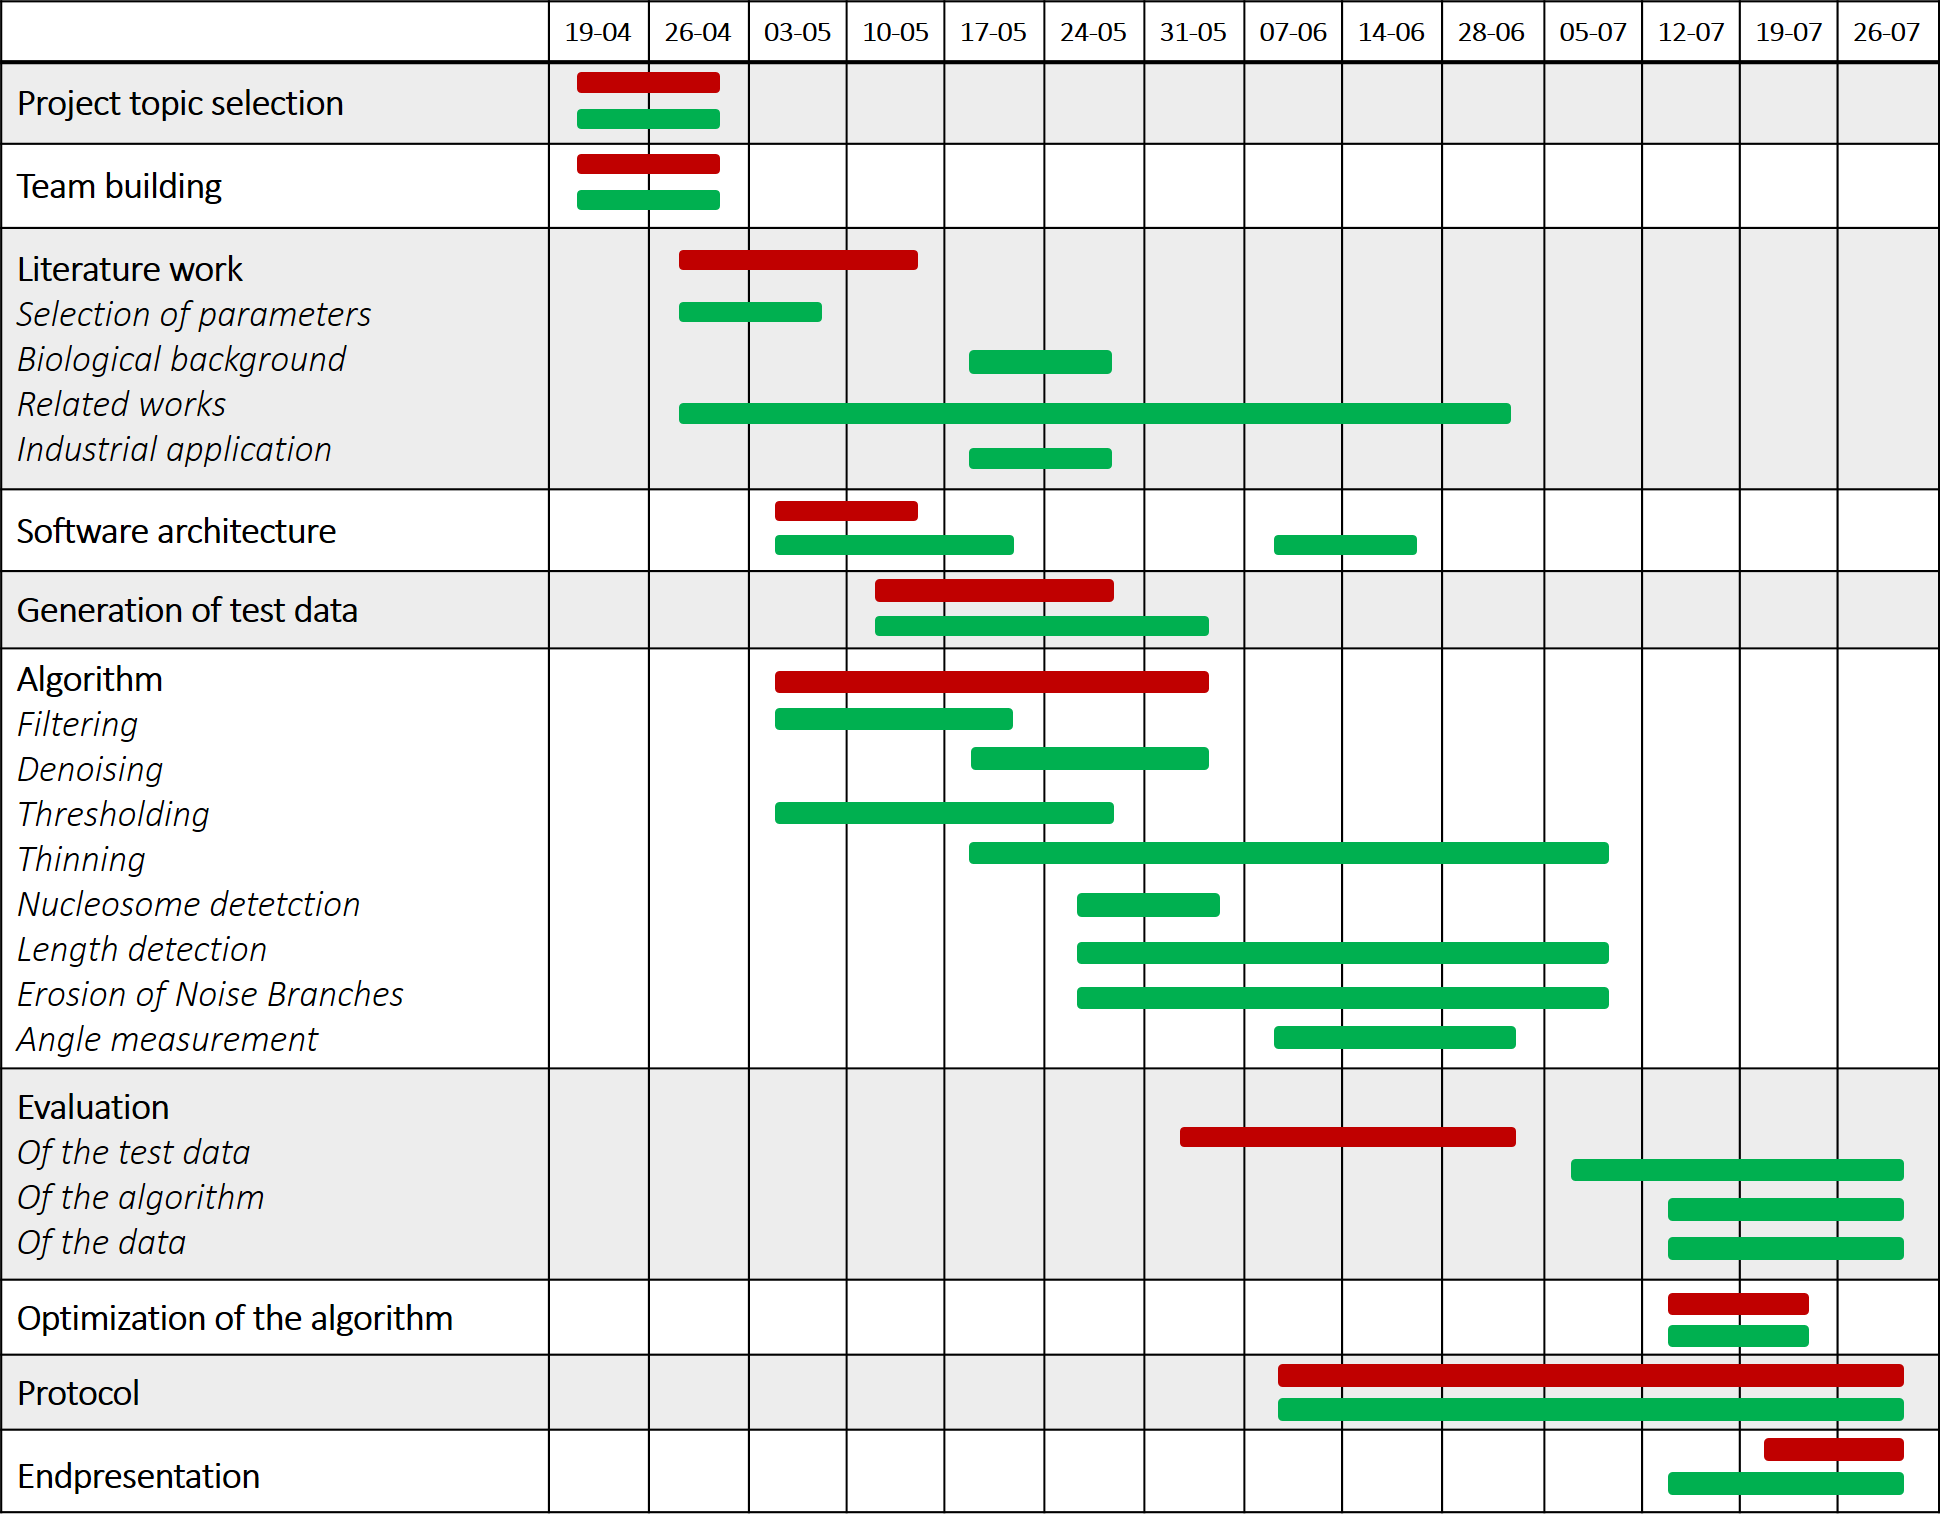
\includegraphics[width = \textwidth]{timeline2.png}
\end{center}
\caption{The expected needed amount of time for each subsection (red) and the actual needed amount of time (green).}
\label{fig: timeline} 
\end{figure}

\begin{abstract}
This report summarizes ...

\end{abstract}

\section{Introduction}\label{sec: Introduction}
\subsection{Motivation}\label{sec: Motivation}


\subsection{AFM}\label{sec: AFM}
Since its invention in 1982 by IBM scientists Gerd Binning and Heinrich Rohrer, atomic force microscopy (AFM) has found widespread applications in various fields ranging from semiconductor science to polymer physics. The simplicity of the underlying concept allows for implementation in a variety of challenging experimental setups including high-energy physics  \cite{fischbach2001new} and live cell biology  \cite{evans2007forces}. The AFM technology has particularly been used not only to obtain high-resolution topographic images (with resolution of up to 1 nm) but also to measure extremely low forces that occur for example during molecular interactions. In this way, major achievements, like first topologies of single atoms and small molecules and their connecting electron bonds, have been made possible  \cite{hoffmann2001direct}.As AFM is a non- destructive imaging technique and large fields of view can be scanned on appropriate time scales, it has found more and more application in the study of living cells and organisms (Figure \ref{fig: phage genome}). Here, it enables even for high resolution studies of the interactions between single cell membrane receptors and ligand drugs \cite{willemsen2000biomolecular}. Moreover, as nanotechnological approaches are becoming increasingly popular, AFM has gained attention for quality control purposes in industry and academia. 

However, automated evaluation of AFM images has remained challenging, especially when highly diverse biological structures, such as DNA molecules, are studied. Mostly because high background and varying morphologies hinder accurate automated evaluations. We here present an image processing algorithm, designed for automated quantification of AFM data to further study DNA histone interactions in higher throughput. 

\begin{figure}[htb]
\centering
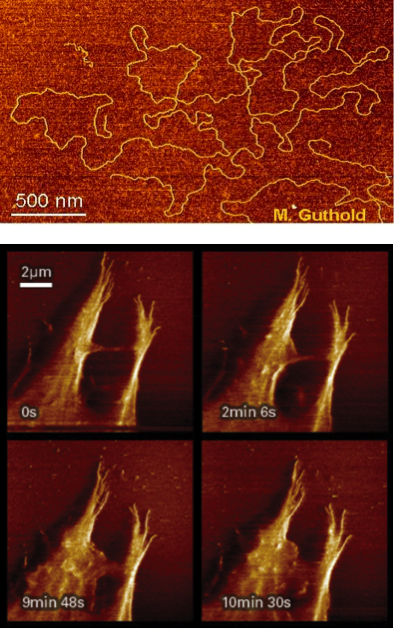
\includegraphics[width = 0.5\textwidth]{Figure1}
\caption{(Top) AFM image of a complete $\lambda$ phage genome with single strand resolution. Colors represent cantilever tip deflection \cite{image11}. (Bottom) AFM image of a living cell showing filopodia rearrangement. Colors represent cantilever tip deflection \cite{image12}.}\label{fig: phage genome}
\end{figure}

\subsubsection{Concept}
The heart of an AFM setup consists of a sharp silicon tip with an ending radius of curvature of up to 1 nm attached to a flexible micro cantilever (Figure \ref{fig: afm setup}). 

\begin{figure}[htb!]
\centering
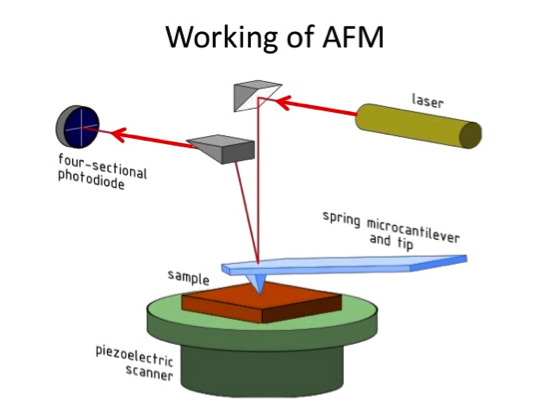
\includegraphics[width = 0.75\textwidth]{Figure2}
\caption{Schematic representation of an AFM setup with optical path of the laser beam in red and xy-controllable Piezo scanner \cite{image2}.} \label{fig: afm setup}
\end{figure}

The cantilever is mounted onto a Piezo controlled z-stage for precise lifting and dipping. With this, the cantilever tip is brought into (close) contact to the surface to be examined. The tip is then further scanned over the surface with constant z-stage deflection and thereby bended by topographic heterogeneities of the sample according to the mechanics described by Hook for simple springs. To precisely measure and amplify these minimal deflections, a focused laser beam is projected onto the cantilevers reflecting top. Redirected onto a four photodiode detector, x- and y- deflection of the elastic cantilever can be recorded as potential differences between pairing photodiodes. Small bendings are thereby amplified by the laser deflection and can be used to compute topographic images. Although being extremely simple, high resolutions can be achieved that are mostly limited by the tips radius and shape (Figure \ref{fig: atom resolution}).

\begin{figure}[htb!]
\centering
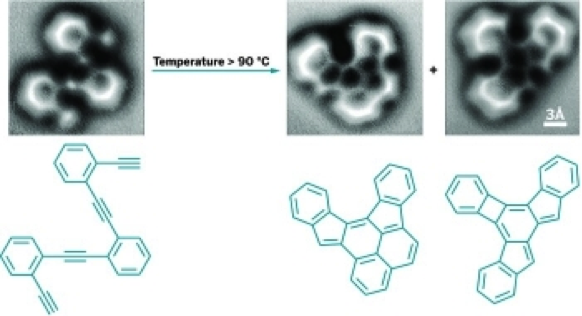
\includegraphics[width = 0.9\textwidth]{Figure3}
\caption{Single atom resolution AFM image and corresponding structural formula of an enediyne compound before and after induction of cyclisation by heating \cite{image3}.}\label{fig: atom resolution}
\end{figure}

However, to preserve the integrity of the examined specimens, which is of particular importance when observing living systems where harsh perturbations are likely to cause artifacts, the AFM is run in a so called tapping mode \cite{binnig1986atomic}. Here, an alternating current is applied to the supporting Piezo element thus oscillating the cantilever over the surface. By this, the tip-surface interaction is minimized and sample can be scanned with less interference.  
The core setup has been further modified and extended to even measure intermolecular forces \cite{hinterdorfer2006detection}. For this, the cantilever tip is slowly approached to a surface. At a specific distance, electrostatic forces will lead to an attraction of the tip and thus a bending of the cantilever. The kinetics of this bending are characteristic for differing molecular interactions \cite{cappella1999force}. By attaching molecules of interest to the AFM tip, specific interaction between these and molecules located at a surface can be measured. Using this concept, the interplay between drug molecules and G-protein-coupled receptors on cell surfaces could be quantified \cite{radmacher1997measuring}. Furthermore, by using conductive tips, the electric properties of materials were studied, an approach that has found wide applications in semiconductor and microprocessor science \cite{lang2004conducting}. 

%Noteworthy, AFM is a non-optical imaging technique that records topographic features of surfaces and not their optical properties. Intensities depicted in AFM images thus correspond to height values (in commonly used TIFF formats scaled between 0-255) rather then photon counts, as in most other microscopy images. Furthermore, image contrast corresponds to surface topography gradients and not to optical density, photon phase drifts or fluorophore emission gradients like in convention optical microscopy setups. 

\subsection{Epigenetics and Histones}\label{sec: Epigenetics and Histones}
Genetic information is mostly encoded within the DNA sequence and its modular components known as genes. However, during the last decades epigenetic mechanisms that regulate genetic information processing, have been recognized as key players in gene regulation. To date, several mechanisms of epigenetic regulation have been found in eukaryotic cells \cite{bird2007perceptions}. Two of the most prominent examples are DNA methylation and chromatin rearrangement.  While methylation is a direct chemical modification of DNA that leads to impaired recognition by DNA interacting proteins \cite{cuozzo2007dna}, chromatin remodeling mechanisms are versatile \cite{jenuwein1998set,gottschalk2009poly,lin2007role}. Here, the accessibility of specific sequences which are crucial for DNA processing are altered. The central elements of chromatin structures are large heteromeric protein complexes known as histones \cite{marino2005histone}. These highly alkaline proteins are exclusive to eukaryotic cells and some archaea, where they act as spools around which DNA can bind.  In this way, histones do not only alter DNA accessibility but also condense the genetic information within the nucleus, a critical steps especially during cell division. 

\subsubsection{Chromatin and Histone Structure}\label{sec: Chromatin and Histone Structure}
Histone complexes are formed between five major components, the histones proteins H1/H5, H2B, H2A, H3 and H4 \cite{marino2005histone}. The histone core is formed between H2A, H2B, H3 and H4 while H1/5 is known to serve as a linking element. The core histones exist as homodimers; all possessing a histone fold domain that is crucial for the interaction between the different dimers. This domain is comprised of three alpha helices that interact as handshake motifs with corresponding domains on the dimer partner. Thus, the histone complex is an octameric aggregate with an approximate diameter of 63 Å where 147 DNA base pairs can wrap around in 1,65-left handed turns. The histone protein H1 binds to the entering and exiting DNA strand thereby stabilizing the DNA histone complex. H1 is also crucial for the formation of higher order chromatin complexes as it mediates the arrangement of histone fibers in which several histone-DNA complexes pair to highly condensed chromatin (Figure \ref{fig: chromatin structure}). 

\begin{figure}[htb]
\centering
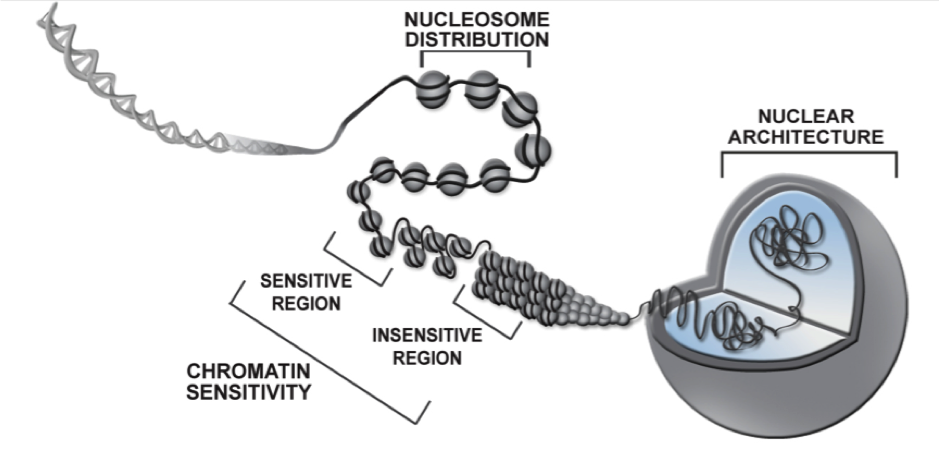
\includegraphics[width = 0.9\textwidth]{Figure4}
\caption{Chromatin structure from a single DNA double helix (left) to the fully evolved nuclear DNA architecture (right). DNA bound single histones are depicted in their modification sensitive conformation, where epigenetic mechanisms regulate gene transcription, and their insensitive condensed form \cite{image3}. }\label{fig: chromatin structure}
\end{figure}

\subsubsection{Histone Modifications}\label{sec: Histone Modifications}
Together with DNA methylation, chemical modifications of histone complexes are a key process in epigenetic regulation as with this, interactions between DNA and nuclear proteins such as transcription factors, polymerases or other regulatory elements can be altered \cite{mersfelder2006tale}. As histones represent complex macromolecular structures, the possible chemical modifications are diverse and yet not fully understood. However, some key players have been identified. Most modifications occur at the tails of histone proteins H3 and H4, which protrude from the DNA-histone complex \cite{lorch1987nucleosomes} (Figure \ref{fig: crystal structure}). 

\begin{figure}[htb]
\centering
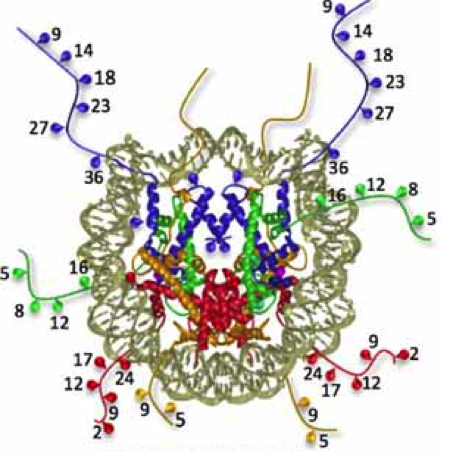
\includegraphics[width = 0.5\textwidth]{Figure5}
\caption{Crystal structure of a histone complex with a modeled double helical DNA strand wrapped around. Colors represent histone dimers (H2A yellow, H2B red, H3 blue, H4 green). Numbers correspond to amino acid sequence position and show frequent modification sites \cite{hansen2010histone}. }\label{fig: crystal structure}
\end{figure}

Here, acetylations, methylations, phosphorylations, ubiquitinations and citrullination have been reported. Additionally, the histone core can also be modified leading to highly complex modification patterns as several modification combinations can occur. By this, either the direct interaction between the DNA and a histone is sterically hampered or the modification acts as a recognition element for other regulatory proteins. For example, lysine acetylation in histone complexes is responsible for the loss of one positive charge and therefore reduces the electrostatic interaction strength to the negatively charged DNA backbone \cite{ozdemir2005characterization}. Therefore, acetylated histones are thought to form less condensed and thus more accessible chromatin structures. On the other hand, gene promoter regions that are bound to non-acetylated histones are known to be responsible for gene down regulation. Another prominent example for histone modification is lysine methylation. Here, up to three methyl groups can be added to a lysine residue at the histone tail. Although this does not diminish the positive lysine charge and thus no direct inhibition of the DNA-histone complex formation is observed (even if the small methyl groups slightly sterically alter this interaction), it serves as a recognition motive for other nuclear responsive elements with Tudor or PHD domains \cite{schotta2004silencing}. The underlying mechanisms appear to be extremely sensitive, as opposite effect between mono- and demethylation have been reported \cite{kourmouli2004heterochromatin}. 
Some well-studied histone modifications that promote gene transcription are triple methylation of H3 lysine 4, which mostly occurs in the promoter region of highly transcribed genes \cite{krogan2003paf1}, and triple methylation of H3 lysine 36, which is frequently observed in the gene bodies of upregulated genes as it recruits histone deacetylase thereby ensuring proper gene transcription \cite{strahl2002set2}. Prominent examples for modifications that repress gene transcription are trimethylation at lysine 27 of H3 \cite{cao2002role}, which induced histone acetylation, and trimethylation of H4 lysine 20 \cite{schotta2004silencing}. 
Hence, histone modification is a generally accepted epigenetic mechanism to regulate gene transcription, where the interaction strength between histones and DNA is of major importance. Mutations within histone complexes that alter this interaction have been associated with various diseases like cancer and chronic inflammations \cite{sawan2010histone}. 

\subsection{Histone Complexes by AFM}\label{sec: Histone Complexes by AFM}
As DNA-histone configuration is of major importance for epigenetic regulation, a profound understanding of the regulatory mechanisms and crucial structural features that conquer this interaction is highly desirable and of special interest for drug design. Here, the AFM technology is preferentially suited to study the molecular configuration with sufficient resolution. AFM is not only able to easily resolve single DNA strands but also to image the volume of single DNA-histone complexes (and thereby the number of DNA turns per histone) and the entering/ exiting angle of bound DNA, which gives insides into the bonding strength between DNA and histone. 
An automated evaluation of DNA structure is not only of interest to study DNA-protein interaction but also to evaluate cancerogenic compounds that alter the DNA architecture. Here, correlations between the cancerogenicity and the geometrical deformation of the compound bound DNA have been observed \cite{japaridze2015influence}. Therefore, quantitative screening of pharmaceutical compounds for their ability to influence DNA structure with AFM resolution could be highly interesting for toxicity studies. 
Moreover, many modern technologies used within the life science sector are based on DNA molecules. For example DNA bound antibodies have been used for immunohistochemical stainings where a DNA bound fluorophore enhances the fluorescence signal \cite{chen2015expansion}. Other applications include DNA micro arrays to study and compare gene expression \cite{adomas2008comparative}. Here, DNA molecules with specific gene complementary sequences are spot printed onto glass cover slips to quantify the amount of specific cDNA present in probes. This widely used technique can monitor slight changes in gene expression. However, quality control of the microarrays themselves has remained challenging. Specialized ventures already test for DNA microarray quality by AFM imaging but are yet not able to provide single DNA strand resolution as automated evaluation of this has been elusive \cite{dokukin2011towards}. With the here presented algorithm we tackle current restrictions in DNA-protein interaction analysis and DNA morphology quantification by AFM. 
\subsection{Related Work}\label{sec: Related Work}
The analysis of AFM images can be categorized into manual, semi-automatic and automatic approaches. Since manual image analysis were human operators draw manually the backbone of DNA filaments is very time consuming and error-prone, we focused on a fully automatic analysis without any supervision. In semi-automatic image analysis approaches, the threshold had been set manually or the initial and/or final point of a DNA filament was set by a human operator  \cite{wiggins2006high},  \cite{marek2005interactive},  \cite{cassina2016effects}.

Automatic image analysis predominantly focussed on the determination of the contour length of DNA filaments  \cite{spisz1998automated},  \cite{sanchez2002accuracy},  \cite{sundstrom2012image},  \cite{marturelliautomated}. The steps of the algorithms are very similar and will be explained below. The contour length is defined as the polymer’s length at maximal physical extension  \cite{rivetti2001accurate}.  Some research groups also considered the curvature or the spatial orientation of DNA filaments  \cite{ficarra2005automated},  \cite{ficarra2005automatic}. 
Doyen et al. used an automated approach for nucleosome recognition according area and height criteria and free DNA length determination of the nucleosomes.

The main steps of DNA contour length determination are first the generation of a binary image, then the skeletonization of traced DNA fragments, and then the length measurement. Many papers are referring to additional optional steps which are not necessary depending on which algorithms were implemented for the thinning step. In the following sections the single steps of the algorithms are explained. 
\subsubsection{Filtering}
In order to reduce the noise, one apply filters before generating the binary image. The filters are either 3x3 mean filters  \cite{rigotti2005quantitative} or 3x3 median filters  \cite{ficarra2005automatic},  \cite{ficarra2002automated} or a Gaussian filter and an adaptive filter  \cite{ficarra2005automated}. 

\subsubsection{Segmentation}
The generation of a binary image is based on a thresholding algorithm which is either determining the threshold globally or locally, depending on the method. Global thresholds are only considering the individual grey value of a pixel, whereas in local thresholding, the neighbourhood of a pixel is critical as well  \cite{weszka1978survey}. A neighbourhood of a pixel consists of four or eight pixels. They can be included in the thresholding process by calculating the mean or median of the grey values. Since local thresholding methods are very CPU-intensive, most studies use global thresholding algorithms. Their thresholds mostly depend on the pixels’ intensity values, whereas in one case a global threshold of 0.2 nm was used  \cite{sanchez2002accuracy}. Finding the optimal threshold, where only valid fragments and no background are considered, is a challenging task. Ficarra et al. \cite{ficarra2005automated}, \cite{ficarra2005automatic}, \cite{ficarra2002automated} use the Ridler method \cite{ridler1978picture}, a method based on a grey value histogram which iteratively determines the optimal threshold. Spisz et al. \cite{spisz1998automated} use two different thresholding techniques. The first technique is based on two Gaussian distributions fitted to the fore- and background grey values and finds the optimal threshold in between those distributions  \cite{gonzales1987wintz}. The algorithm cannot be applied to all AFM images, therefore they implemented a second method which finds the minimum threshold where the number of recognized fragments (blobs) does not change  \cite{russ1992image}. Setting a too high threshold leads to the fragmentation of DNA filaments (see Figure \ref{fig: blobs}).

\begin{figure}[htb]
\begin{center}
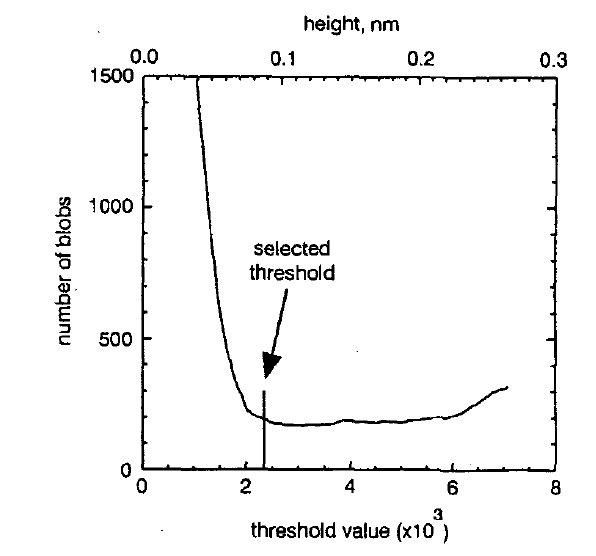
\includegraphics[width = 0.7\textwidth]{Segmentation_histo}
\end{center}
\caption{Determination of an optimal threshold. For each threshold the resulting number of blobs were calculated. The optimal threshold is the minimal threshold value at which the number of blobs does not decrease any further. \cite{russ1992image}}
\label{fig: blobs} % you need to include this to reference the figure afterwards
\end{figure}

Another option is to consider a pixel’s neighbouring intensity values instead of the pixel’s intensity value  \cite{marek2005interactive}. By doing so, filtering and segmentation are combined into one step.


\subsubsection{Thinning}
The thinning step is used in order to erode the fragments to skeletons with the width of one pixel which is necessary for the length determination. The fast parallel thinning algorithm by Zhang and Suen iteratively removes pixels from each fragment if they possess all the conditions of removal  \cite{ficarra2005automated},  \cite{ficarra2002automated},  \cite{ficarra2005automatic},  \cite{spisz1998automated},  \cite{zhang1984fast},  \cite{marturelliautomated}. This algorithm does not remove corner pixels and removes valid end pixels with a high probability. The algorithm by Brugal and Chassery \cite{brugal1977new},  \cite{sanchez2002accuracy} iteratively removes connected pixels in a specific order. The end pixels are not affected by the algorithm, therefore no end pixel restoring is necessary. Sundstrom et al. do not describe their thinning algorithm but only emphasize that it is necessary to convert the fragments into skeletons with a width of one pixel  \cite{sundstrom2012image}.


\subsubsection{Removal of Corner Pixel}

During thinning invalid corner pixels can be included into the DNA skeleton which results in a longer distance in corner areas. Those pixels are not real compartments of the DNA structure and hence need to be removed  \cite{sanchez2002accuracy},  \cite{ficarra2002automated},  \cite{spisz1998automated}.

\subsubsection{Removal of Objects Across the Image Boundary}

For fragments at the image boundary a complete analysis is not possible. Therefore, such fragments have to be excluded from further steps. Ficarra et al. used a 8-pixel neighbourhood for the detection of such objects. If the connectivity in the neighbourhood was not interrupted at the image boundary the object has been removed  \cite{ficarra2005automated},  \cite{ficarra2005automatic}. 

\subsubsection{Pruning}

After thinning some short branches often remain at the skeletons. The reasons are impurities in the sample or noise close to the DNA fragment. Sundstrom et al. \cite{sundstrom2012image} referred to a master thesis by Silvio Cirrone CHECK who transformed the skeleton into a graph. Thus the problem was formulated as a graph optimization problem to cope with short branches. Otherwise, the removal of the branch pixels is necessary. Ficarra et al. \cite{ficarra2002automated},  \cite{ficarra2005automated} created a mask to distinguish between unbranched and completely detected cases, branches, critical cases, and corners. Spurious branches have the characteristic of being much shorter than the fragment. This feature is used to identify such branches and to delete them recursively.  



\subsubsection{Removal of Invalid Fragments}

In this step, critical molecules are removed before analysing their length. Spisz et al. \cite{spisz1998automated} carry out this step before thinning the fragments. Fragments are defined as invalid when they are overlapping with other fragments or with themselves, when they are in a closed circle conformation, when the endpoints are not distinguishable, when more than two endpoints are detected and when they exceed a user-defined size  \cite{spisz1998automated},  \cite{ficarra2005automated},  \cite{ficarra2002automated},  \cite{ficarra2005automatic}. Ficarra et al. used for the removal of such invalid fragments different masks. For overlapping molecules the masks shown in Figure \ref{fig: Masken} have been used  \cite{ficarra2005automated}.

\begin{figure}[htb]
\begin{center}
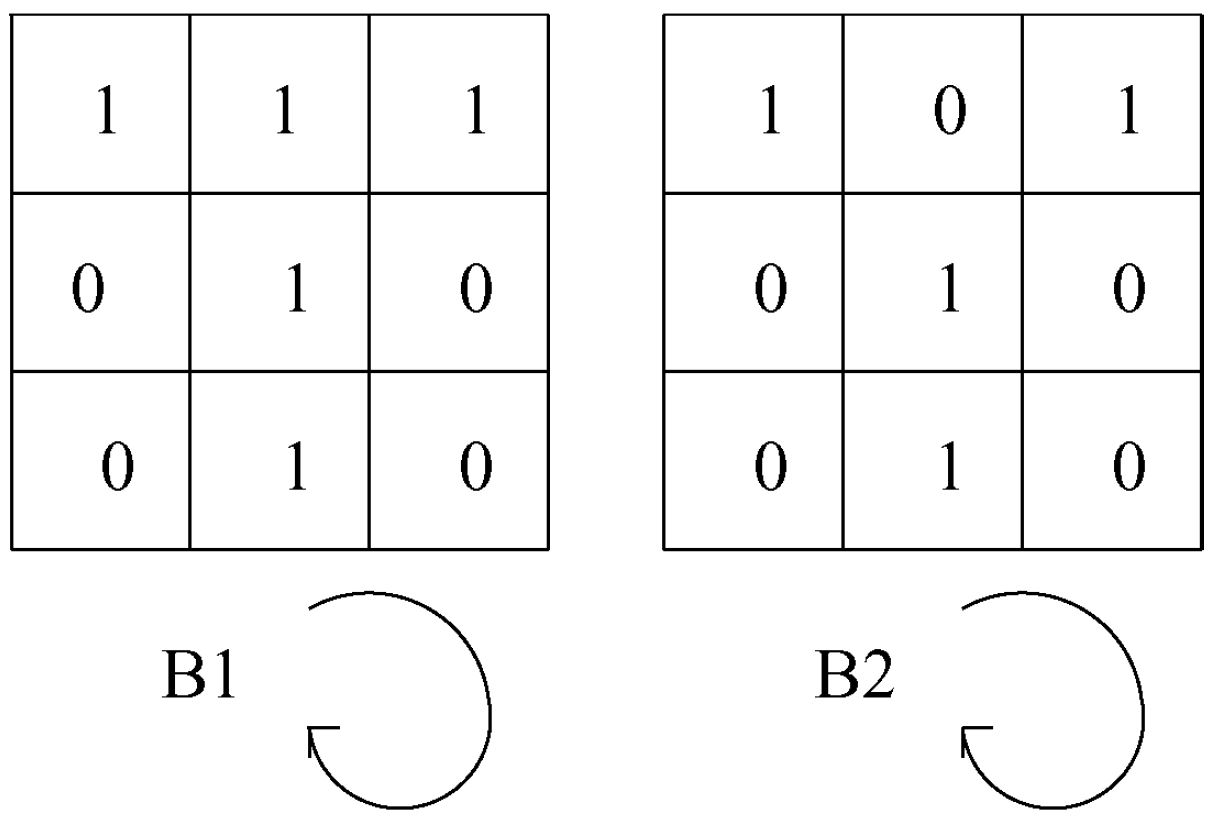
\includegraphics[width = 0.7\textwidth]{Masken}
\end{center}
\caption{Masks for identifying overlapping molecules. \cite{ficarra2002automated}}
\label{fig: Masken} % you need to include this to reference the figure afterwards
\end{figure}



\subsubsection{Pixel Restoring}

Pixel at the skeleton ends only need to be restored if they were erroneously deleted during thinning of the fragment. The end pixels of each backbone are virtually extended in the direction of the last two pixels. If the new possible end point was part of the fragment before, the pixel is restored  \cite{spisz1998automated},  \cite{ficarra2005automated},  \cite{ficarra2002automated},  \cite{ficarra2005automatic}.



\subsubsection{Length Determination}

The determination of the length of the DNA skeletons is achieved by estimating the contour length which is defined as the polymer’s length at maximal physical extension  \cite{rivetti2001accurate}.  During digitization, the exact contour is lost. Anyhow, the accurate determination of the contour length is for many applications crucial. The Freeman estimator is the most commonly used method to determine the length  \cite{spisz1998automated},  \cite{marturelliautomated}. When the fragment is reduced to a skeleton with the width of one pixel, the connection between one and another pixel can be represented by eight directions (Figure \ref{fig: freeman}A). The Freeman estimator is adding the distance between the connected pixels from one endpoint to another. Even connections thus with vertical or horizontal direction are counting as 1, odd connections with diagonal connections are multiplied by 1.414. \\

$ L_{F} = n_{e} + \sqrt{2} n_{o}= 1.000n_{e} + 1.414n_{o}  $ 

\hspace{0,2cm}
 
$ L_{F}$: \begin{footnotesize} 
DNA contour length determined by the Freeman estimator
\end{footnotesize}  

$ n_{e}$: \begin{footnotesize} 
 number of even connections
\end{footnotesize} 
 
$ n_{o}$: \begin{footnotesize} 
 number of odd connections
\end{footnotesize}  \\

Even though the Freeman estimator is often used, it overestimates the DNA length by approximately eight percent  \cite{sanchez2002accuracy}. Rivetti and Codeluppi \cite{rivetti2001accurate} analysed in 2001 six different algorithms to determine the contour length, one of them being the Freeman estimator. 
Secondly, they tested the most probable origin estimator, which similar to the Freeman estimator computes an ($n_{e}$, $n_{o}$) characterization. This algorithm calculates the contour length as a function of the number of egde pixels, number of pixels on diagonal edges and of the area \cite{pan1991root}, \cite{dorst1987length}. \\

$ L_{MPO} = \sqrt{(n_{e} + n_{o})^{2} + n_{e}^{2}} $

\hspace{0,2cm}

$ L_{MPO} $: \begin{footnotesize}
DNA contour length determined by the most probable origin estimator
\end{footnotesize} \\

Much better results were obtained for the Kulpa estimator which is derived from the Freeman estimator. The coefficients of even and odd pixels minimize the error when measuring the length of long fragments.\\

$ L_{K} = 0.948n_{e} + 1.343 n_{o} $

\hspace{0,2cm}

$ L_{K} $: \begin{footnotesize}
DNA contour length determined by the Kulpa estimator
\end{footnotesize} \\

The corner count estimator considers additionally to the number of even and odd connections the number of different code pairs, so called corners (Figure \ref{fig: freeman}B)  \cite{vossepoel1982vector}. The coefficients were found by least-square fitting  \cite{yang1994methods}.  \\


$ L_{C} = 0.980n_{e} + 1.406 n_{o} - 0.091 n_{c} $

\hspace{0,2cm}

$ n_{c} $: \begin{footnotesize}
number of corners
\end{footnotesize} \\


\begin{figure}[htb]
\begin{center}
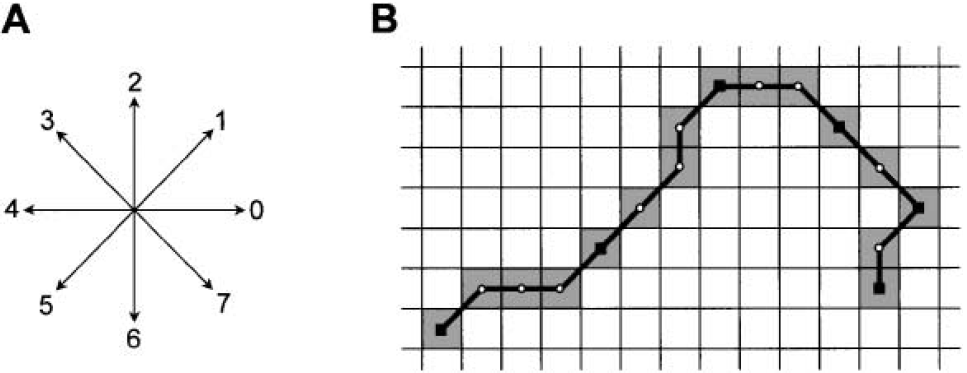
\includegraphics[width = 0.7\textwidth]{freeman}
\end{center}
\caption{(A) Scheme of the eight connected chain code. (B) Example of a fragment skeleton containing 16 pixels (grey grid elements). The chain is connected by 15 codes, from the left to the right chain the codes can be written as 100111210077756. There are six even codes ($ n_{e} $) and nine odd codes ($ n_{o} $). The total number of corners ($ n_{c}$) is six.}
\label{fig: freeman} % you need to include this to reference the figure afterwards
\end{figure}

As fourth estimator Rivetti and Codeluppi tested an estimator where the backbone was primarily smoothed by using polynomial fitting. The coordinates of each pixel where thereby adjusted. The polynomial degree was three and the moving window consisted of five points since the estimation with this combination were very close to the real length. \\ 

$ L_{PF} = \sum_{i=1}^{n-1} \sqrt{(x_{i+1}-x_{i})^{2} + (y_{i+1}-y_{i})^{2}} $

\hspace{0,2cm}

$ L_{PF} $: \begin{footnotesize}
DNA contour length determined with polynomial smoothing
\end{footnotesize} \\



The last algorithm included in their analysis was the edge chain algorithm which was originally implemented to measure the length of the roots of plants. It can be applied for other objects with relatively constant width and draws chords along the object edge to determine its perimeter. \\

$ L_{ECA}=\dfrac{P+\sqrt{P^{2}-16A}}{4} $

\hspace{0,2cm}

$ L_{ECA} $: \begin{footnotesize}
DNA contour length determined by the edge chain algorithm 
\end{footnotesize} 

$ P $:\begin{footnotesize}
perimeter
\end{footnotesize} 

$ A $:\begin{footnotesize}
area
\end{footnotesize} \\

Rivetti and Codeluppi generated synthetic data similar to their AFM images with DNA fragments of different length and tested the estimators while knowing the exact length of the synthetic filaments. The estimations with the Kulpa estimator, the corner count estimator, and with polynomial smoothing were significantly closer to the real length of the filaments than the estimates generated by the other three estimators. The overestimation of the Freeman estimator was confirmed  \cite{rivetti2001accurate}.



Ficarra et al. \cite{ficarra2002automated},  \cite{ficarra2005automated} calculated the molecule length using the Euclidean distance which was integrated over all consecutive pixels of the molecule. For calculation the pixel coordinates were recalculated as weighed average by using a weight factor k.\\


$ X_{P} = k(x_{p-1}-x_{p})+x_{p}+k(x_{p+1}-x_{p}) $

$ L_{P+1,p}= \sqrt{(X_{p+1}-X_{p})^{2}+(Y_{p+1}-Y_{p})^{2}} $

\hspace{0,2cm}

$ X_{P} $:\begin{footnotesize}
weighed average x coordinate
\end{footnotesize}

$ k $:\begin{footnotesize} 
single weight factor
\end{footnotesize}

$ L_{p+1,p} $:\begin{footnotesize} 
modified distance between the points with coordinates x and y
\end{footnotesize}\\




\section{Methods}\label{sec:Methods}
\subsection{Test Data Creation}\label{sec:Test Data Creation}
Missing: Description of the images we are using
\subsubsection{Manual Analysis}\label{sec:Manual Analysis}
To annotate and evaluate the results of the algorithm the open source program ImageJ (2.0.0-rc-46/1.50g) was used. Therefore, the features from a sample of objects or from whole images, were analyzed manually with the tools of ImageJ.
For the objects, which were single DNA-strands and mono nucleosomes, the location and the couture length were determined. For nucleosomes, also the angle between the two DNA-strands entering the nucleosome core, the approximate area of the nucleosome core and the mean gray value of the nucleosome core were measured.
To annotate the manual data from one object to the results of the algorithm the centre of mass was used. Therefore a binary image was created by thresholding. Then the "Analyze Particle Tool" was used to read out the x-y coordinates of the centre of mass from the different objects. 
All other parameters were determined on the original images. To measure the different lengths, the "Segmented Line Tool" was used. One end of a DNA strand was set as starting point, from which the line-points were drawn centrally through the fragment towards the other end of the fragment. This so called couture length was also measured for mono nucleosomes, by drawing centrally through the DNA and through the approximate center of the nucleosome core (figure). For mono nucleosomes, however two lengths were determined. The second length was the distance between the approximate center of the nucleosome core and the end of the shorter of the two entering DNA-strands.
The entry/exit DNA-strand angles of mono nucleosomes were measured by using the three point selection "Angle Tool" of ImageJ. Figure illustrates that the entry/exit DNA-strand angles can be determined in two different ways. In that context, $\alpha_1$ and $\alpha_2$ were measured on different mono nucleosomes for the test data evaluation.
$\alpha_1$ was measured by connecting the two entry/exit points of the nucleosome with the approximate center of the nucleosome core. For the determination of $\alpha_2$, the two DNA-axes at the nucleosome core were traced. The angle between the two DNA-axes was then measured at their intersection point.
The approximate area and mean gray value of nucleosomes were determined by manually fitting an elliptical structure to the nucleosome cores with the "Oval Selection Tool" of ImageJ.
Besides single DNA strands and mono nucleosomes, the locations of special objects were recorded. The special objects were intersecting DNA-fragments/nucleosomes, self-intersecting DNA-fragments/nucleosomes, objects on the edges of an image and undefined objects. To increase objectivity, test data were measured from four different persons.

\begin{figure}[h!]
\centering
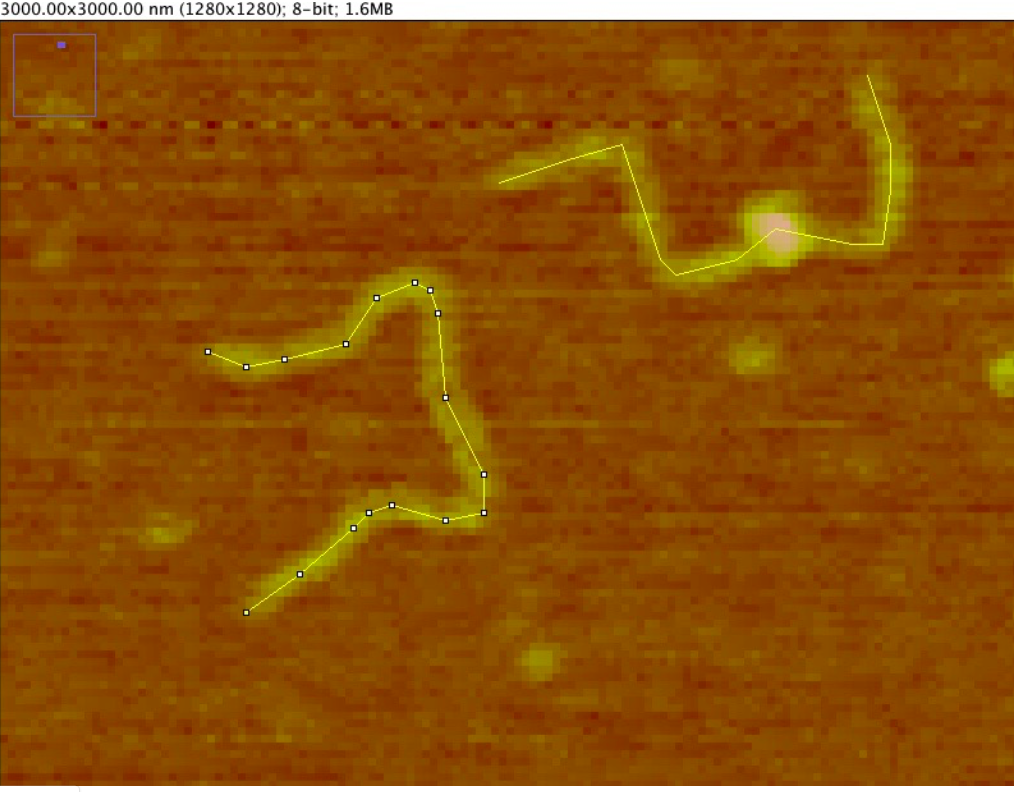
\includegraphics[width = 0.5\textwidth]{coutureLength.png}
\caption{Couture length measurements of DNA and nucleosomes
The contour length of DNA and nucleosomes were measured with the "Segmented line tool" of ImageJ. The white bars indicate the selected points. The lines have been traced centrally through the DNA fragments from one end point to the other end point.}
\label{fig: couture length}
\end{figure}

\begin{figure}[h!]
\centering
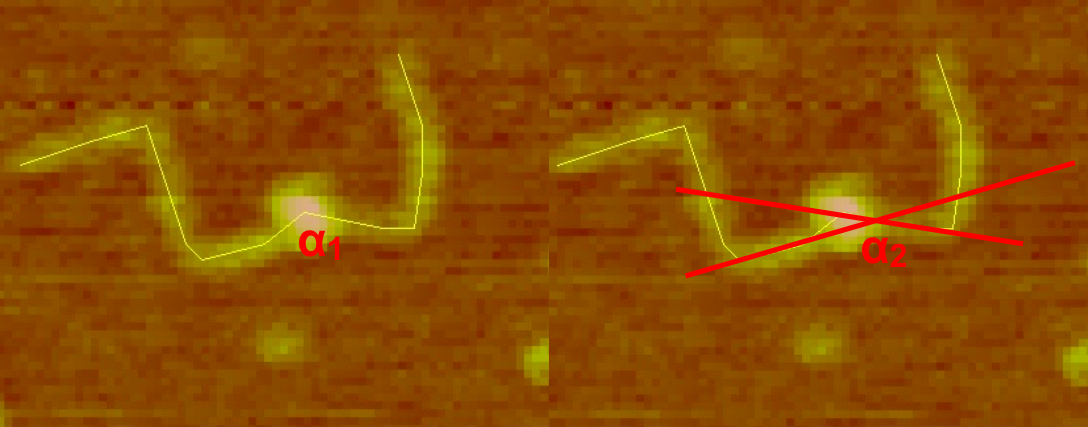
\includegraphics[width=0.7\textwidth]{angleMeasurement.png}
\caption{Angle measurement of mono nucleosomes
The figure shows two possible angles $\alpha_1, \alpha_2$ which can be measured between the two entering DNA strands of an nucleosome. $\alpha_1$ is the angle between the entry/exit points of the DNA with respect to the approximate center of the nucleosome core. $\alpha_2$ is the angle between the DNA-axes (red lines), which are crossing the entry/exit sites of the nucleosome core, with respect to their intersecting point.}
\label{fig: angle measurement}
\end{figure}
\newpage
\subsection{Software Architecture}\label{sec:Software Architecture}
\subsection{Denoising}
\subsection{Filtering}\label{sec:Filtering}
%Although it is common practice to use filtering techniques as a way of preprocessing the data, it was the goal 
At first, one needs to ask why it is necessary to use filtering techniques in the first place, as it is stated in various other papers (insert citation here). Since the goal was to find a most efficient and fast solution, a heuristic approach was proposed which only took object size of (MATLAB) connected components into account.\\
Although this eliminated most of the smaller fragments, and some larger ones, obviously some objects remained that were dirt or impulsive noise. \\
Like (Ficarra et al.) pointed out, a median filter with a 3x3 mask helps eliminating these components quite well, yet there is still room for improvement. Regarding the aspect of very limited available data, it was another aim to maximize the number of sampled strings. Therefore other, less common techniques besides the already tested filters were approached.\\
As it was rather soon apparent that regions with impulsive noise had a rather high frequency in frequency domain, a lowpass filter approach seemed like the way to go.

%\subsubsection{High Pass Filter}\label{sec:High Pass Filter}
%Low frequency noise can occur in AFM images due to vibrations in the operating environment of the AFM. To filter out the low frequency noise a Butterworth high pass filter was implemented. It has a maximally flat frequency response in the pass band.

\subsubsection{Adaptive Lowpass Filter}\label{sec:Adaptive Lowpass Filter}
Firstly, the most prominent example for a lowpass filter is the Gaussian filter. It essentially smoothes the data out, but in a relatively predictive way, since it has a predefined filtering matrix, similar to the median filter. But, since it is not always known just how high the signal-to-noise ratio really is, a simple Gaussian filter might only blur the edges of the outer DNA regions, instead of effectively reducing the amount of stray noise. Rather than simply smoothing the image with a Gaussian filter, the idea was to eliminate regions with high contrast.  \\
Filtering out exactly such high-contrast regions is best achieved in frequency space. The freuquency domain, simply put, transforms the original image data into a decomposition of sinus waves. For the transformation between spatial domain and frequency domain the MATLAB implementation of the Fast Fourier Transformation was used. Without going into further detail, the amplitude of such a frequency representation now gives a comparatively abstract, but nonetheless intuitive, visualisation of such high contrasts as shown in (figure x). \\
As one can easily observe, there is a denser circular area in the image center. This central area represents the lower frequencies which corresponds to a constant image region. This can be seen on every picture of the used dataset but is to be expected in every other dataset as well. The only difference lies in the clear distinction and brightness of the center. Since a classic lowpass filter requires a clipping region as a fixed parameter, it would not work perfectly for every picture because one would inevitably overfit for a certain set of images. Standard circular detection via circular Hough transform has not been able to sufficiently detect this area. \\
It should be mentioned that for non-quadratic images an ellipsoid instead of a circle can be observed. In this case the algorithm differs only in one step, so for consistency and simplicity only the circular case is presented. \\
% The huge improvement of the proposed filter is now an adaption to the low frequency area. In the following section, the method is discussed in detail.

% 02.07 Dennis and Philip
\subsubsection{Description of Proposed Method}\label{sec:Description of Proposed Method}
% -> figure with images might come in later and will be referenced after each processing step.
As input, the method takes an arbitrary grayvalued image which then is transformed to the frequency domain with MATLAB fft2 function. For a representation similar to above a shifting of the result has to be done as well. A detailed description of the frequency functions and their specific useage can be found on mathworks' homepage (insert link). \\
The complex result has then to be transformed into a grayvalue amplitude image in which the imaginary part is thrown out and the real part is visualized as a logarithmic absolute value. Now the result is generally the same as above. \\
For the approximation of the circle it is also necessary to convert the image to a binary image. Since only a rough threshold is really necessary a simple and fast algorithm for thresholding is used (built-in Otsu as described in (reference to Christian)). This rough approximation can be excused due to the clear lack of a distinct circular contour. This also explains why the implemented circular Hough transform (MATLAB imfindcircles) was not able to deliver satisfying results.\\
\\
In the used dataset sometimes a distinct lack of very low frequencies - equaling a sharp (yet only one pixel in width) line in the center - could be noticed. To rule out similar cases in other datasets as well, a 20x20 white rectangle was inserted in the center (see result section for further discussion).
Afterwards a standard erosion with a disk shape is performed. With erosion noise that persists in the binary image is eliminated by fitting these disks around each black pixel and coloring all pixels within this shape black as well. A detailed explanation on how to define structuring elements such as the used disk and the MATLAB imerode function can be found on (mathworks link here) as well. \\
Of the remaining connected objects the circle now represents the largest one. Hence it is filtered out with MATLAB bwareafilt(.., 1, 'largest') which extracts this largest region and the resulting image has only this central part colored in white. To assure a compact center another operation is performed which fills in enclosed black areas within the circular region (imfill(...,'holes')). \\
The remaining spikes at the top and bottom of the cirlce are removed by deleting every row where there are only a certain number of white pixels. To reverse the erosion process and get a representative circle the MATLAB imdilate operation is performed with a disk structure. \\
MATLAB's regionprops function delivers the centroid as well as the minor and major axis length of the object which then is used to calculate an approximation of the actual radius of the circle. Notice that it is also possible to extract an ellipsoid structure from non-quadratic images which will not be described in detail here since it does not differ from the steps for a quadratic image. \\
% 03.07 Dennis
For the radius approximation the following formula is used: (insert formula here) \\
Since the removal of the spikes also flattens the circle a bit, it is important to slightly weight the major axis length a bit heavier.  For the distance to the center a 2D-grid is produced by MATLAB ndgrid, using one grid for the distance in x- and one for the distance in y-direction. Following up on this, the distance to the center point is then calculated by the ordinary circular formula to determine whether a point is within the circle (another formula here).Now evaluationg said formula for each point allows to select the circular region which is then stored as a binary matrix. \\
To finalize the steps, the circular region is "cut out" of the original image by multiplying it with the initial fourier transformed image. Before retransforming the image, an inverse shift has to be done with ifftshift. After using ifft2 to recover a spatial form of the image it is also important to transform it back into a uint8 image, using only the real-valued part of the transform. \\
This can all be put together in one code line, resulting in
\begin{lstlisting}
image = uint8(real(ifft2(ifftshift(image))));
\end{lstlisting}

% changes 03.07 Dennis order swapped with results and comparison
\subsubsection{Advantages over Other Filtering Techniques}\label{sec:Advantages over Other Filtering Techniques}
Before comparing the results of the proposed method it should also be discussed why there was no other filter used instead.
The biggest issue with filtering techniques is that it is hugely dependent on the available dataset. While others (insert papers with AFM image data here) usually have a pretty distinct noise level and try to optimize for this specific set of images, it was the goal to really adapt to various datasets. For different qualities of AFM pictures, and especially for different resolutions and cutout sizes, results may vary although done by the same instrument or person. \\
(Ficarra et al.) use three distinct filtering techniques for the preprocessing step: A 3x3 median filter, an adaptive Wiener filter and a high-pass filter. As for the median filter, the proposed method was also used as described (later or earlier) in this paper. As a side note it should be mentioned that the median filter has good results for filtering out sudden peaks of noise but is rather inefficient with larger dabs of noise in an image. \\
The mentioned Wiener method wasn't pursued any further for the following reasons. For one, it works best for a constant noise level which isn't given in all datasets what ultimately let to the design of an own method. Also it is very suitable to clean up the inital data which isn't as much a requirement to this algorithm since it has a fully devoted step of image denoising before filtering out anything. Hence another denoising step would only disturb the image more than it would help remove further artifacts. \\
The problem of the high-pass filter was a bit more subtle. Although it is helpful in providing sharper edges for the later detection of DNA strings, it also attenuates the intensity border between dirt and actual DNA strings (compare section on Histograms). As for the high-pass filter itself, it does the exact opposite of a low-pass filter: Namely sorting out all of the lower frequency in fourier space. The aim of Ficarra et al. was to eliminate noise which was rather low-freuqent but yet again this is a step usually eliminated with denoising in this algorithm. \\
Generally the methods by Ficarra would lead to a much lower rate of actual DNA in the resulting objects and therefore requiring a more subtle decision in whether or not it actually is a DNA string which is currently viewed. By sacrificing a distinct border between the DNA and background, a much lower percentage of noise will be classified as a false positive in the end.

\subsubsection{Results and Comparison}\label{sec:Results and Comparison}
% 8 images as comparison
% compare the changes in the histogram before and after the filtering steps.

\begin{figure}[!htb]
        \begin{subfigure}[b]{0.24\textwidth}
                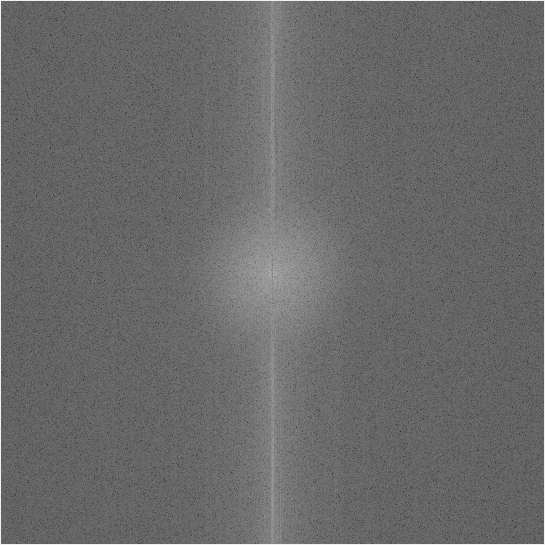
\includegraphics[width=\linewidth]{step1}
                \caption{}
                \label{fig:initial amplitude }
        \end{subfigure}%
        \hspace{\fill}
        \begin{subfigure}[b]{0.24\textwidth}
                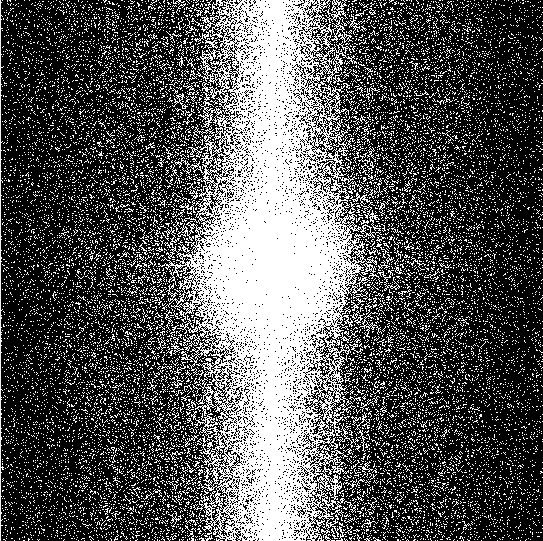
\includegraphics[width=\linewidth]{step2}
                \caption{}
                \label{fig:gull2}
        \end{subfigure}%
        \hspace{\fill}
        \begin{subfigure}[b]{0.24\textwidth}
                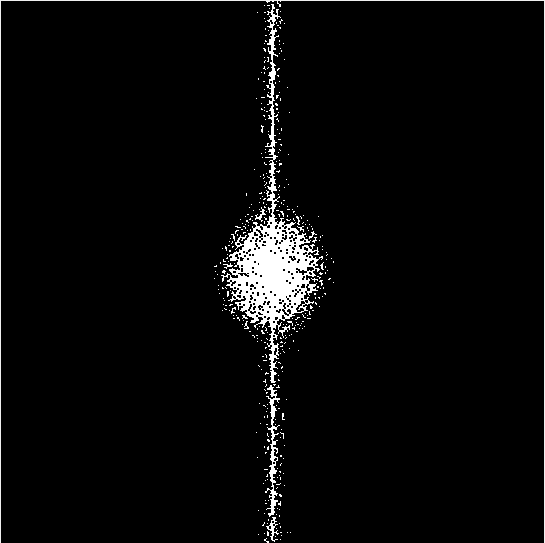
\includegraphics[width=\linewidth]{step3}
                \caption{}
                \label{fig:tiger}
        \end{subfigure}%
        \hspace{\fill}
        \begin{subfigure}[b]{0.24\textwidth}
                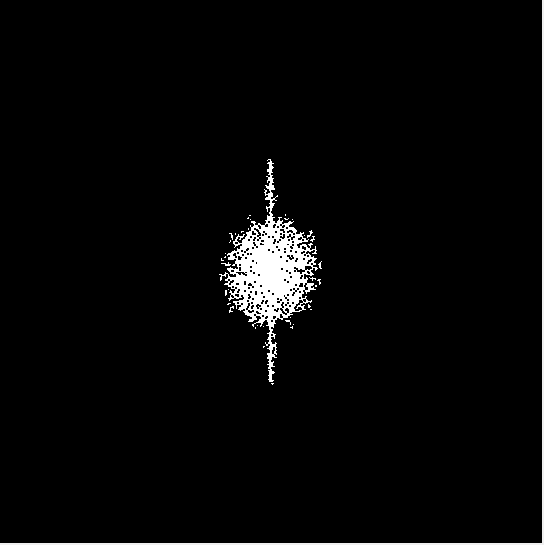
\includegraphics[width=\linewidth]{step4}
                \caption{}
                \label{fig:mouse}
        \end{subfigure}
        \begin{subfigure}[b]{0.24\textwidth}
                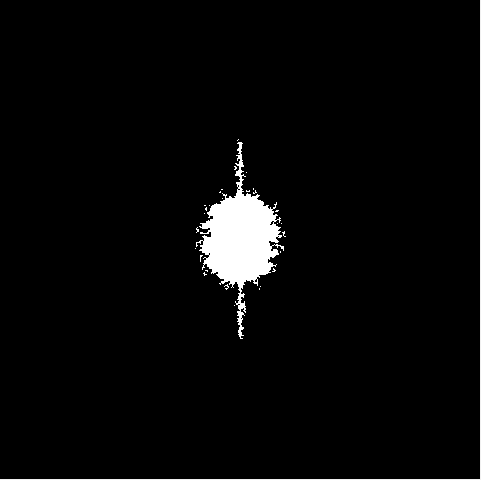
\includegraphics[width=\linewidth]{step5}
                \caption{}
                \label{fig:gull}
        \end{subfigure}%
        \hspace{\fill}
        \begin{subfigure}[b]{0.24\textwidth}
                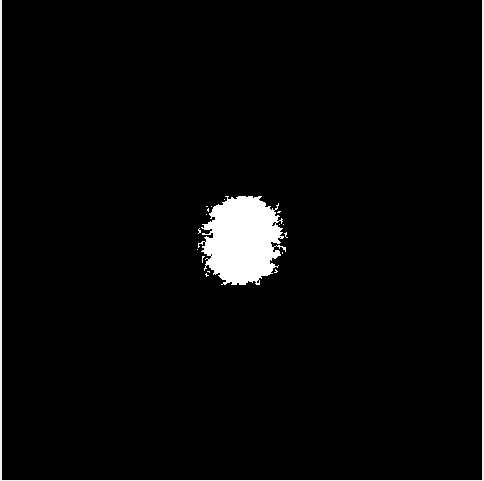
\includegraphics[width=\linewidth]{step6}
                \caption{}
                \label{fig:gull2}
        \end{subfigure}%
        \hspace{\fill}
        \begin{subfigure}[b]{0.24\textwidth}
                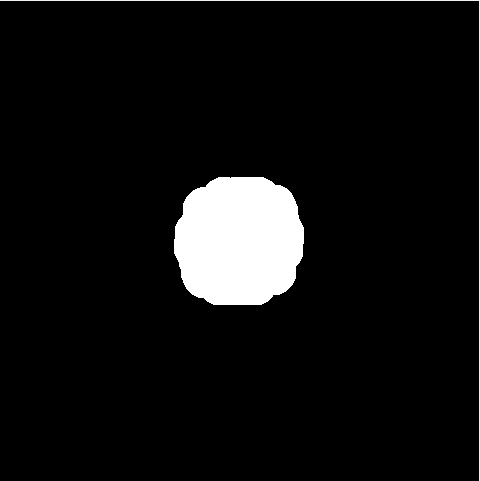
\includegraphics[width=\linewidth]{step7}
                \caption{}
                \label{fig:tiger}
        \end{subfigure}%
        \hspace{\fill}
        \begin{subfigure}[b]{0.24\textwidth}
                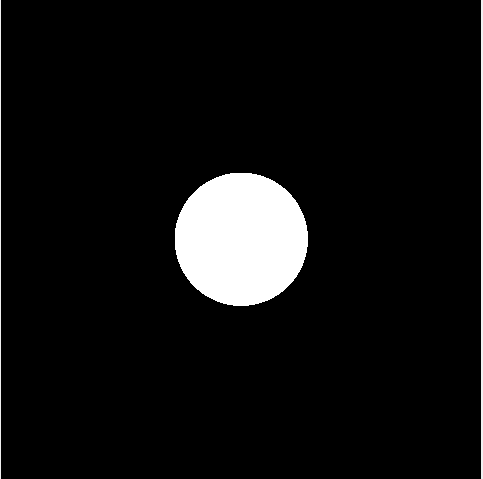
\includegraphics[width=\linewidth]{step8}
                \caption{}
                \label{fig:mouse}
        \end{subfigure}
        \caption{Step-by-step view of circle detection. (a) shows the amplitude representation of the initial fft transform.
(b) is the binary image.
(c) is showing the eroded image with (d) being only the largest connected component.
In (e) holes are filled. for (f) the spurious edges are removed.
Lastly, a dilation is performed in (g) and the resulting circular selection is displayed in (h).}\label{fig:lowpass}
\end{figure}

% 03.07 Dennis initial description and structure
\subsection{Thresholding}\label{sec:Thresholding}
Missing: Explain why thresholding is used.

\subsubsection{Adaptive Thresholding}
The TIFF images often vary in intensity, distribution and scaling of the height profile of the DNA samples. This presents a couple of problems for the thresholding algorithms, such as pollution of some image regions which distort the threshold. As discussed here (\ref{sec:Thresholding}) these issues lead to a false classification of the DNA strands up to completely falsifying the results on this image.
Two sorts of noise persist after the initial pipelining steps  
Opencv Denoising, LowPassFilter and Median Filter (see Section \ref{sec:Filtering}).
\begin{figure}[!htb]
	\begin{subfigure}{0.5\textwidth}
		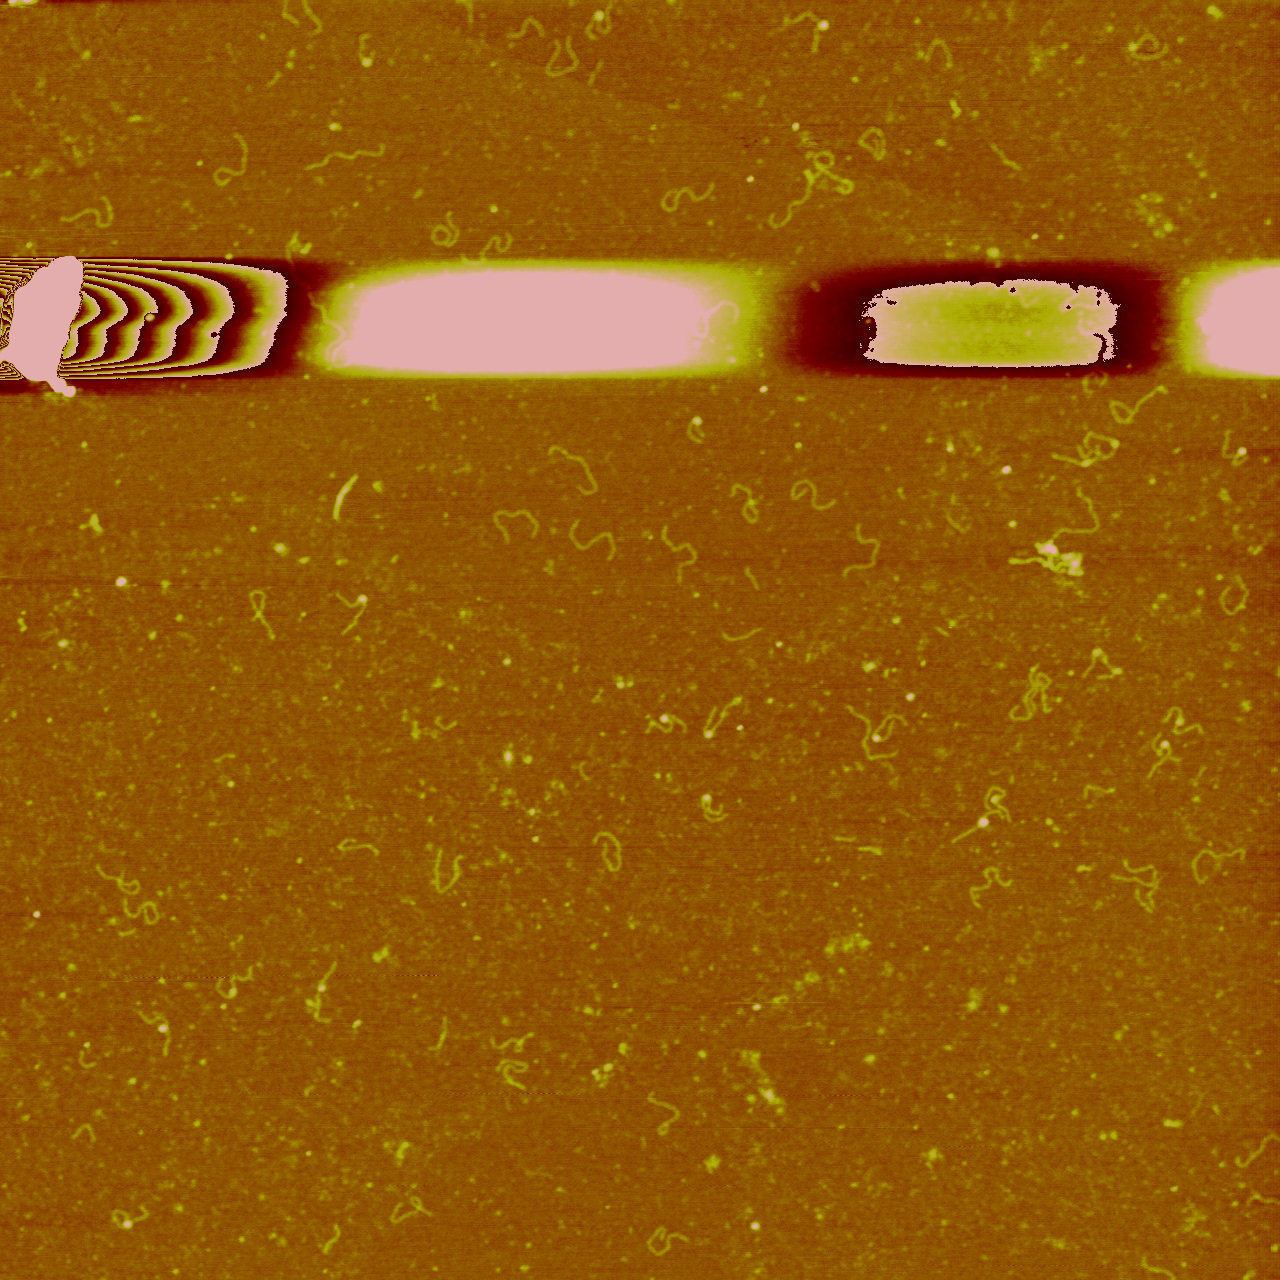
\includegraphics[width=\linewidth]{noise1.png}
		\caption{}
		\label{fig: Noise1}
	\end{subfigure}%
	\hspace{\fill}
	\begin{subfigure}{0.5\textwidth}
		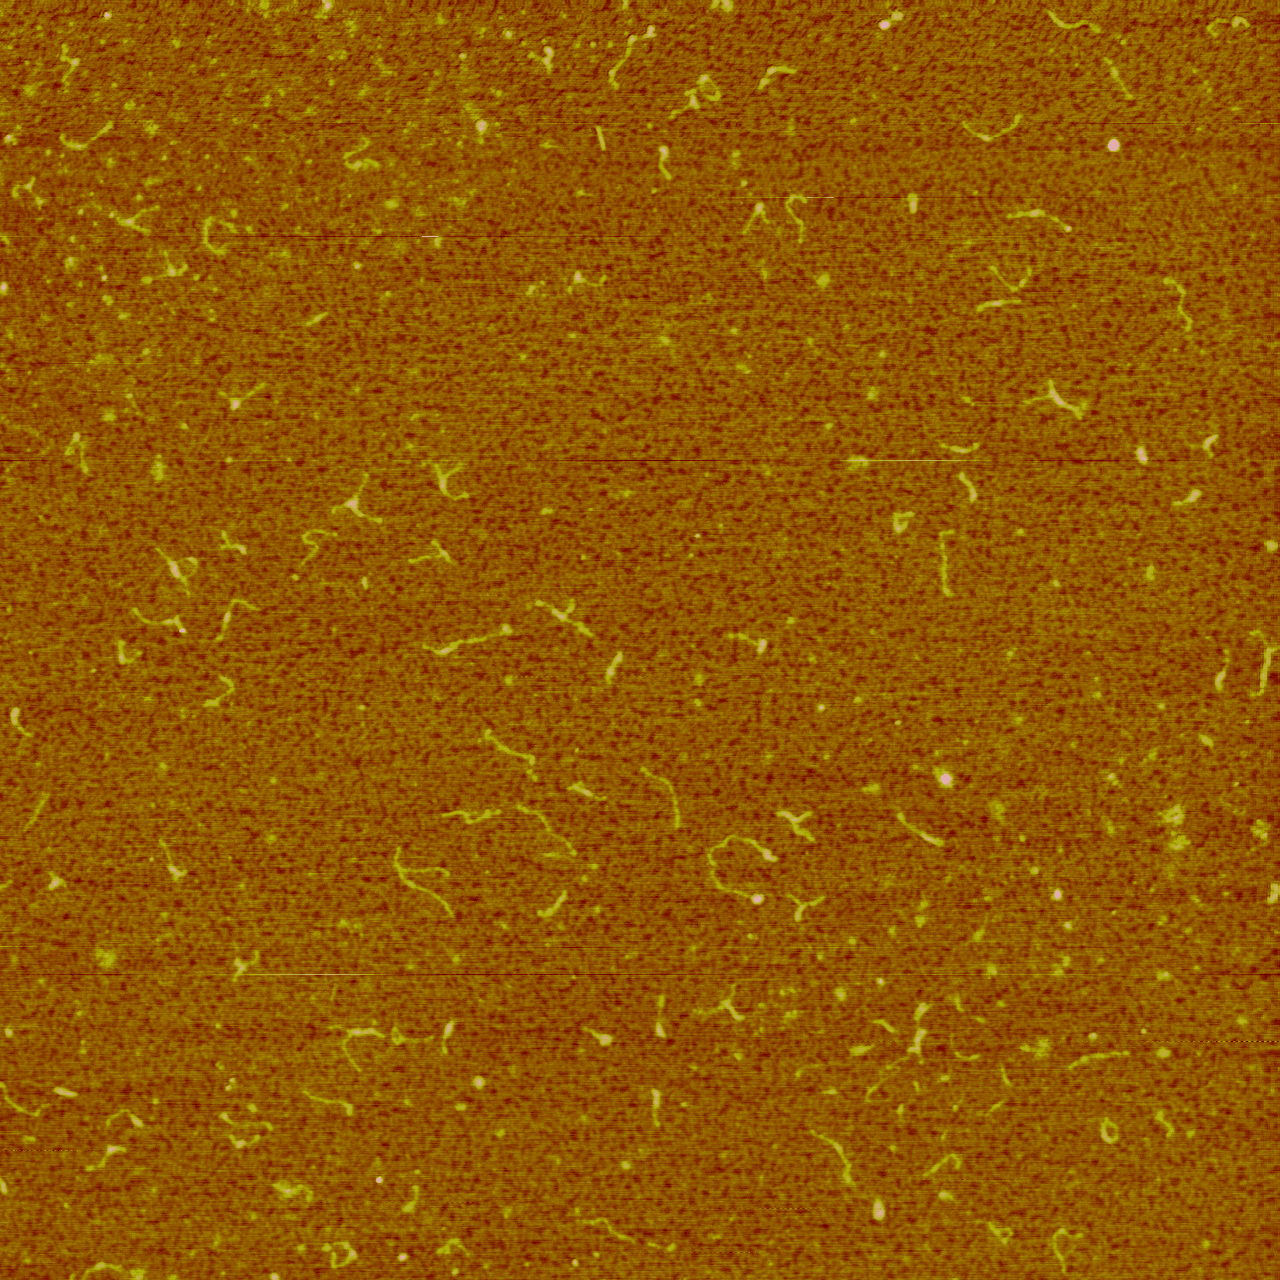
\includegraphics[width=\linewidth]{noise2.png}
		\caption{}
		\label{fig: Noise2}
	\end{subfigure}%
	\caption{(a)Noise Example 1 (b)Noise Example 2}\label{fig:Noise1Noise2}
\end{figure}
\\
The first type of noise as seen in Figure \ref{fig: Noise1} are large distorted regions in the upper value range at an approximate height of 190. If not handled these regions lift the threshold to a level where DNA-strands are missed entirely. 
The second sort of noise seen in Figure \ref{fig: Noise2} consists of small imperfections scattered over the whole image.
Unfortunately the height profile of these imperfections is very similar to the one of the DNA-strands and it is therefore very hard to automatically distinguish between them.
The overwhelming majority of disturbance on the images observed is part of the first type.
The aim of this part of the pipeline is to pre-process the data by three additional steps which treat the outliers in the upper value range and if possible improve detection and removal of scattered noise.

In order to tackle these issues the following three step method is proposed:
\begin{enumerate}
	\item Homogenize the background to provide a consistent and distinguishable layer on which the DNA-strands can be recognized easily.
	\item Identify and remove polluted image regions and outliers in the upper intensity values.
	\item Limit the threshold to an appropriate range.
\end{enumerate}
\subsubsection{Level Background}

Figure \ref{fig:HistThresh} shows a histogram of the height values of a representative original image from the dataset.
In the observed dataset DNA-strands can only be found in an intensity range from about 110 to 160, while nuclei can be found between 160 and 200.


\begin{figure}[!htb]
	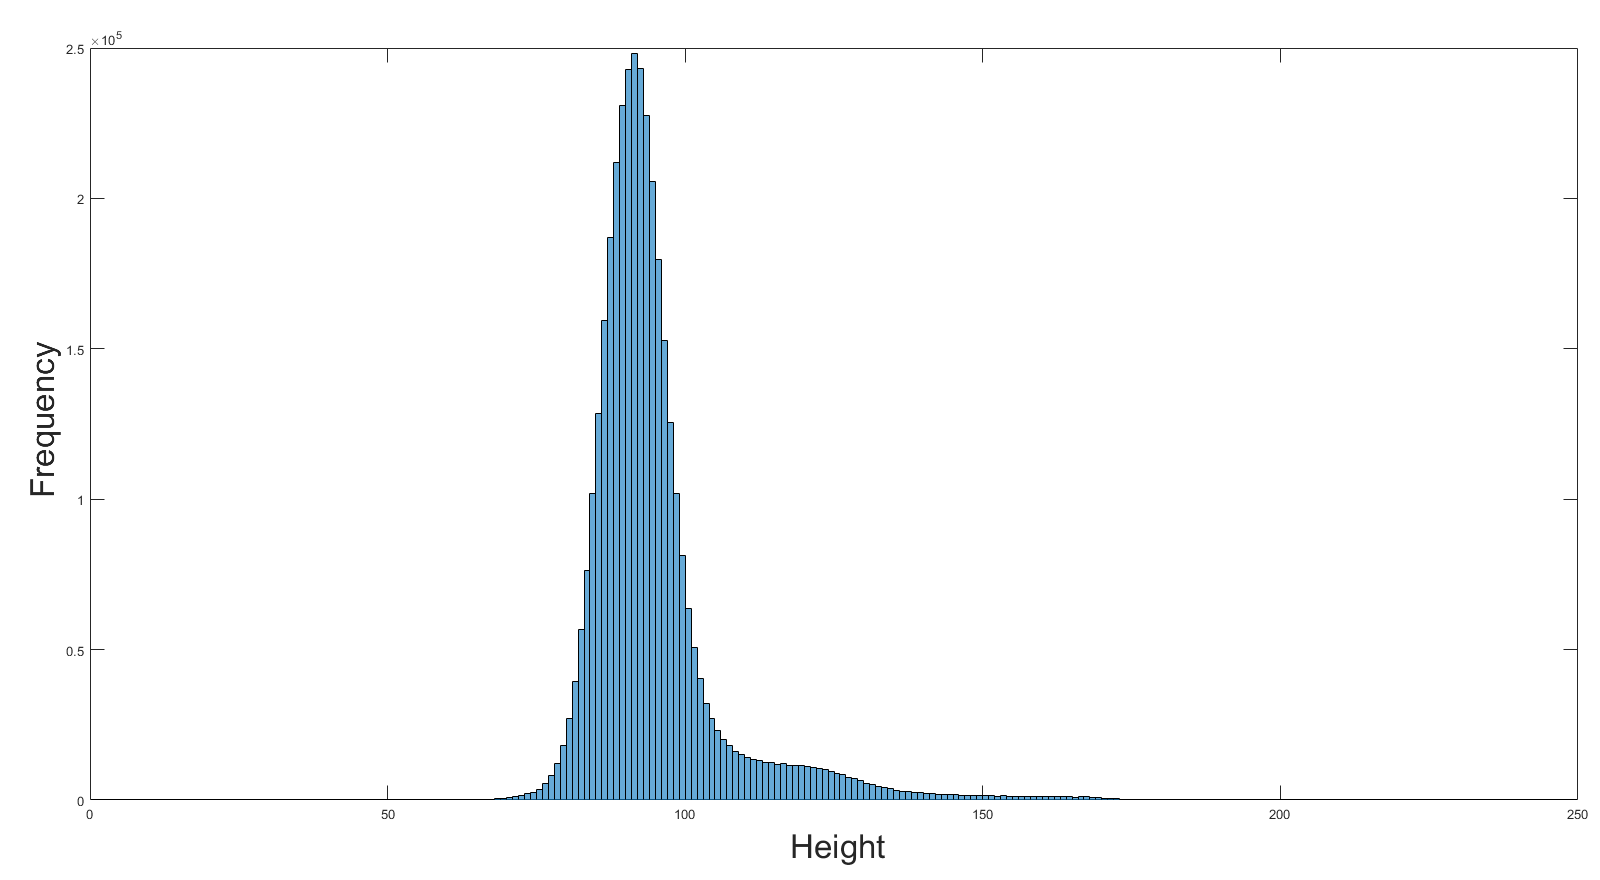
\includegraphics[width=1\linewidth]{histogramOriginal.png}
	\caption{Histogram of TIFF image}
	\label{fig:HistThresh}
\end{figure}
The accumulation point at a value of 95 is distinctive for background noise. 
Therefore, smaller values are set to this boundary.
This approach creates a more consistent background for all images and limits the variation due to noise.
It is important to mention that this method can only be used after the lowPassFilter which smooths the height distribution and thereby guarantees that only noise is removed. If applied to the raw unfiltered image this method will also remove outliers within the DNA-strands which results in perforated DNA objects.
The resulting image shown in Figure \ref{fig:background} yields a more consistent threshold and with that a higher error resistance.


\begin{figure}[!htbp]
	\begin{subfigure}{0.5\textwidth}
		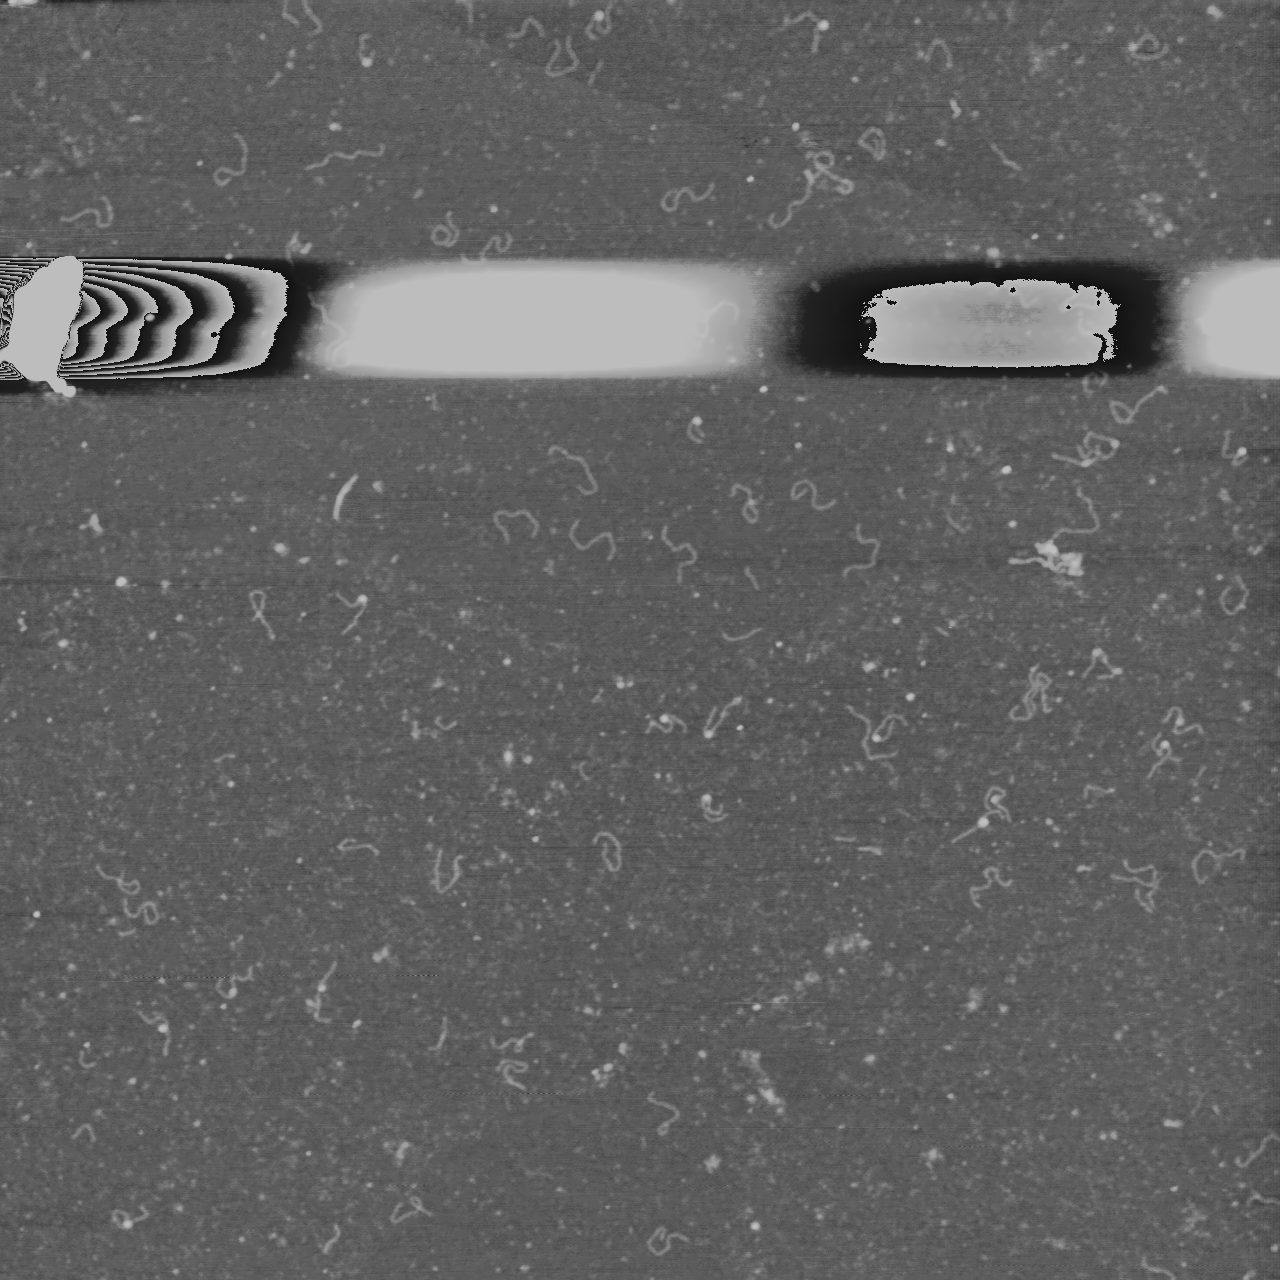
\includegraphics[width=\linewidth]{noise21.png}
		\caption{}
		\label{fig:rawImage}
	\end{subfigure}%
	\hspace{\fill}
	\begin{subfigure}{0.5\textwidth}
		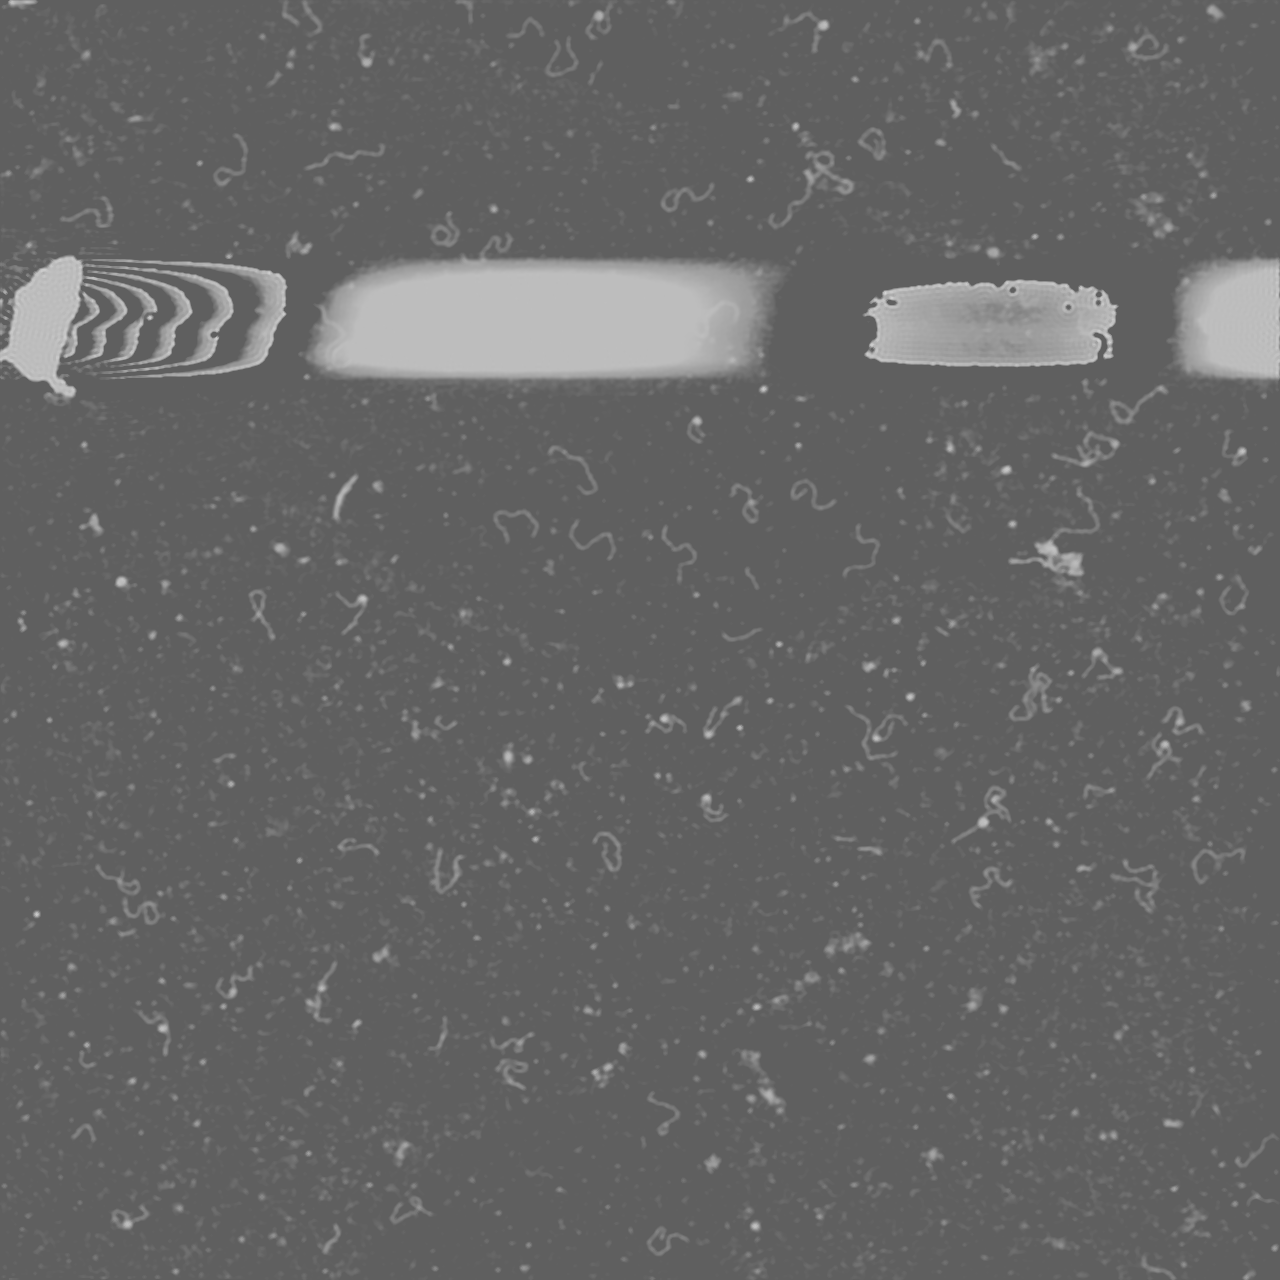
\includegraphics[width=\linewidth]{step21.png}
		\caption{}
		\label{fig:step1}
	\end{subfigure}%
	\caption{(a)Before leveling (b)After leveling }\label{fig:background}
\end{figure}
\subsubsection{Identify and remove outliers}
At first a global threshold algorithm like the Otsu method (see section \ref{sec:Thresholding}) is used to create a binary image.
All objects that could be a DNA object are removed based on size. Now only noise and other non-DNA objects are left.

\begin{figure}[!htb]
	\begin{subfigure}{0.5\textwidth}
		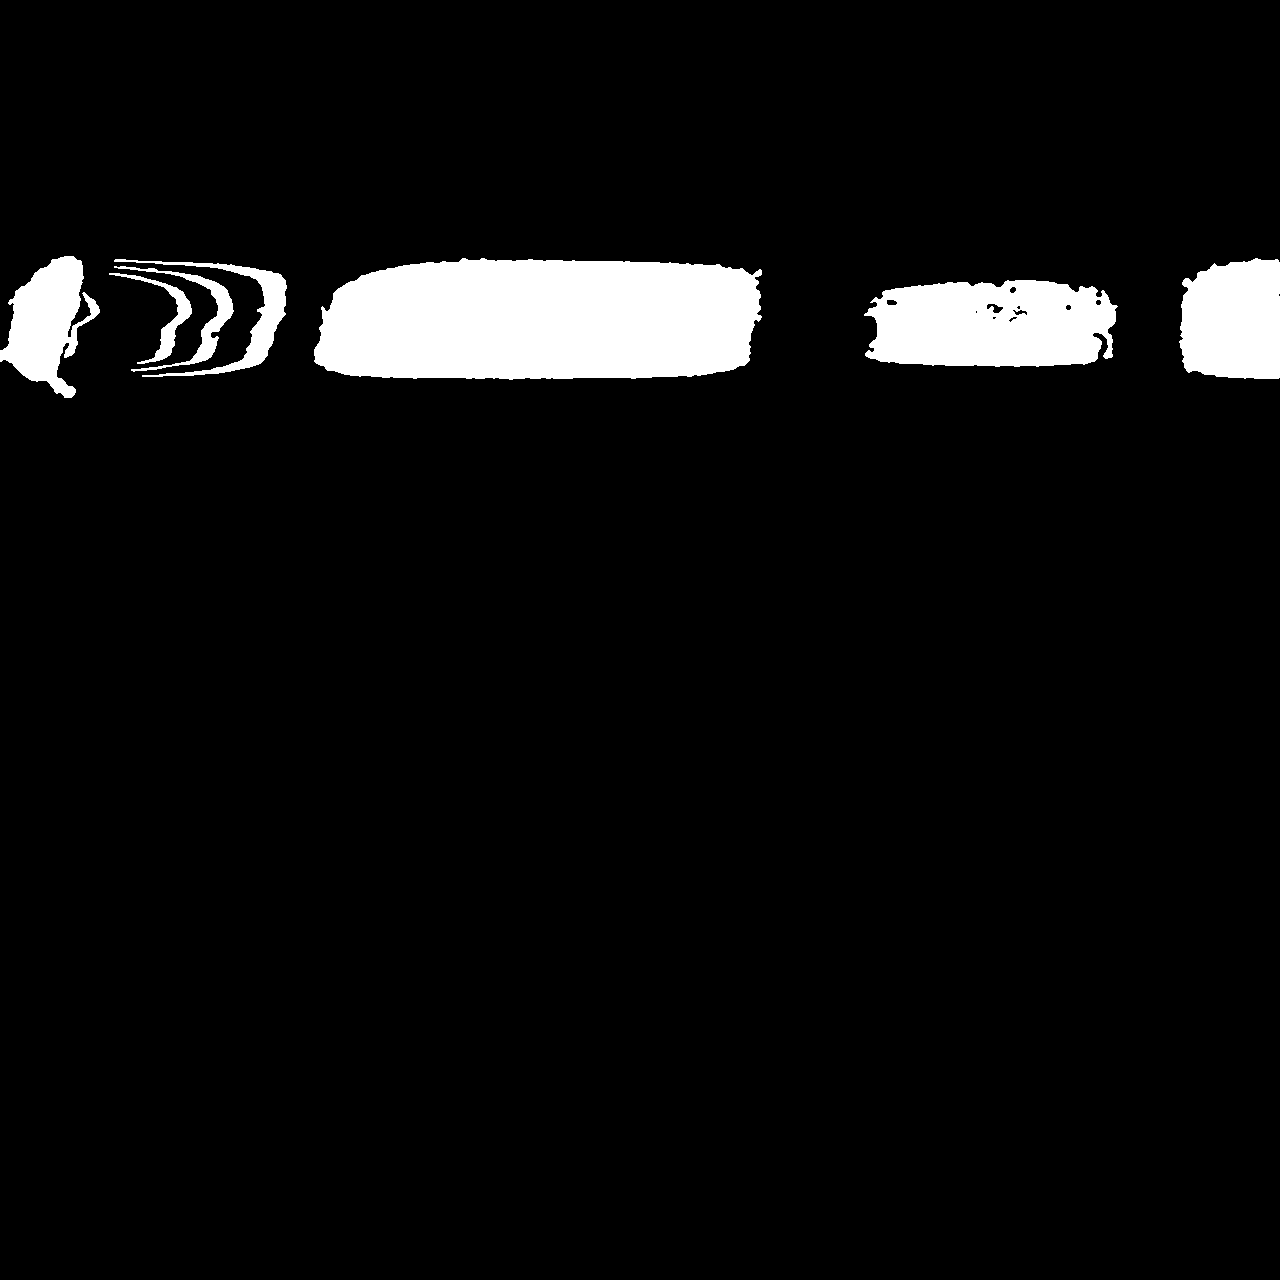
\includegraphics[width=\linewidth]{Maske.png}
		\caption{}
		\label{fig:mask}
	\end{subfigure}%
	\hspace{\fill}
	\begin{subfigure}{0.5\textwidth}
		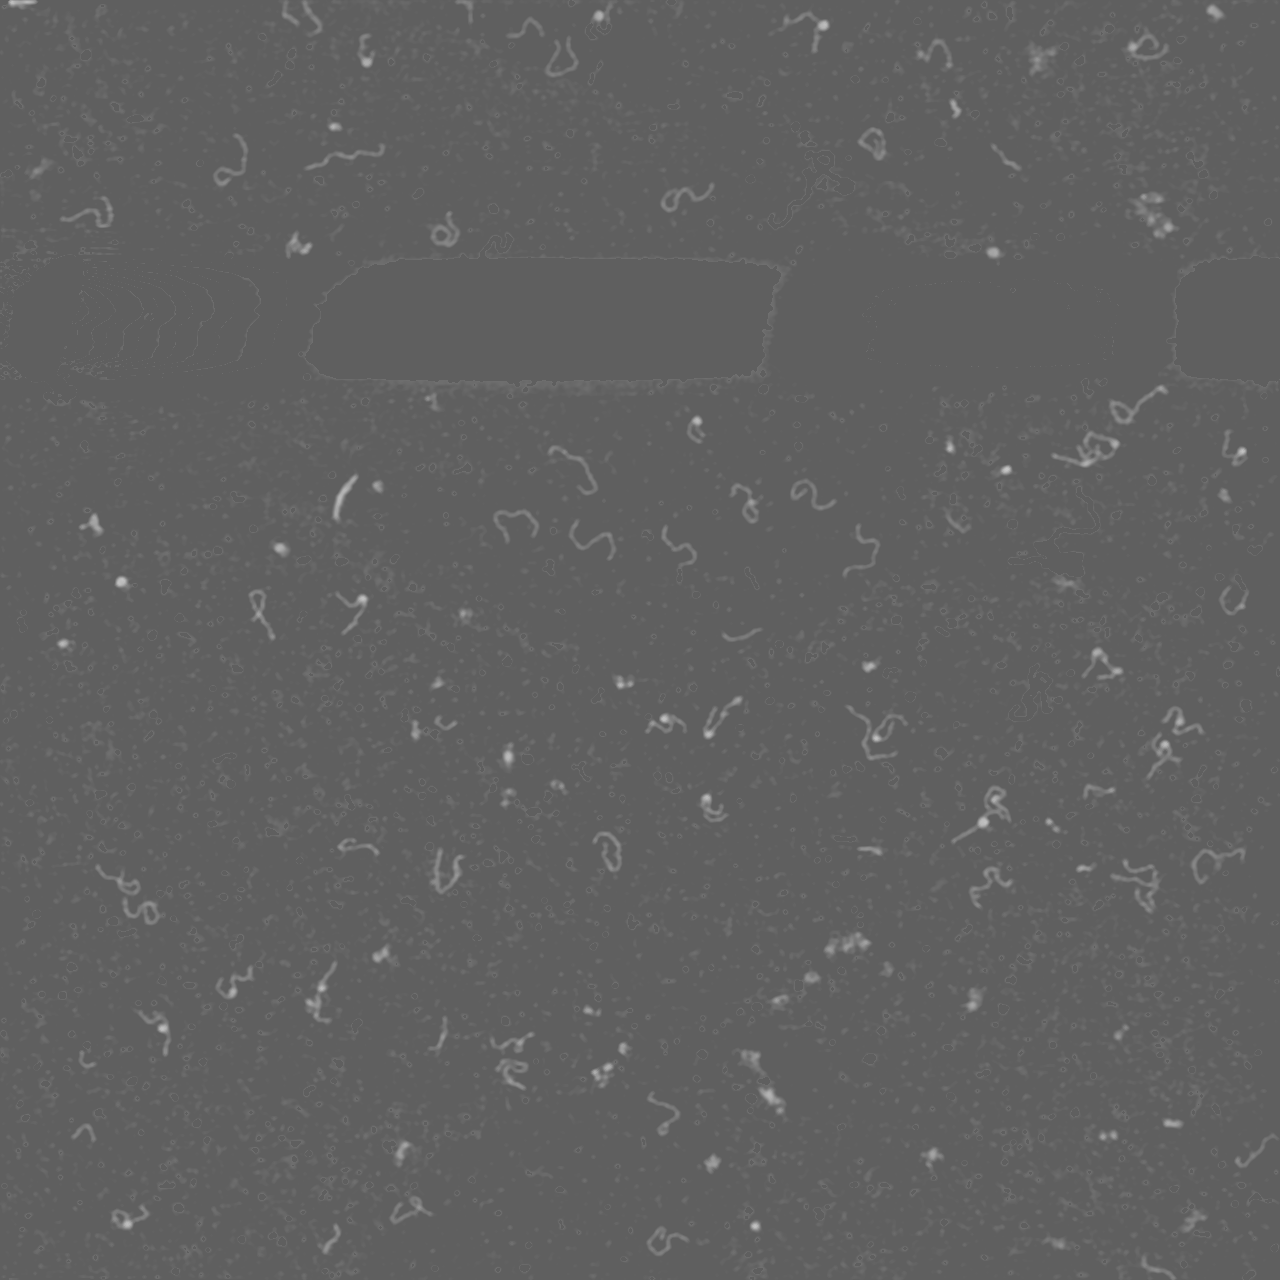
\includegraphics[width=\linewidth]{filtered.png}
		\caption{}
		\label{fig:filtered}
	\end{subfigure}%
	
	\caption{(a)Mask from binary image (b)Mask applied to original image}\label{fig:Process}
\end{figure}
This image is then used as a mask (compare Figure \ref{fig:mask}) which removes all non-DNA objects on the original image from step one.

This means subtract the detected regions on the mask from the original image and set them to the previous determined background level.
The result Figure \ref{fig:filtered} shows how the large outliers are removed and will therefore no longer contribute to the threshold in a negative way.
After this process a second threshold algorithm, in this case the moments threshold (see \ref{sec:Thresholding}), is applied to the original image. 
Duo to the previous steps the new calculated threshold is no longer influenced by background noise or polluted image regions.

In this case the new threshold is now at a intensity value of 111, compared to a intensity value of 135. Figure \ref{fig:compareThresh} shows the improvement in terms of recognized DNA objects on the sample image for type one noise as seen in Figure \ref{fig: Noise1}.
By using this approach it is now possible to analyze pictures with the first type of noise while they had to be discarded entirely before.


\begin{figure}[!htbp]
	\begin{subfigure}{0.5\textwidth}
		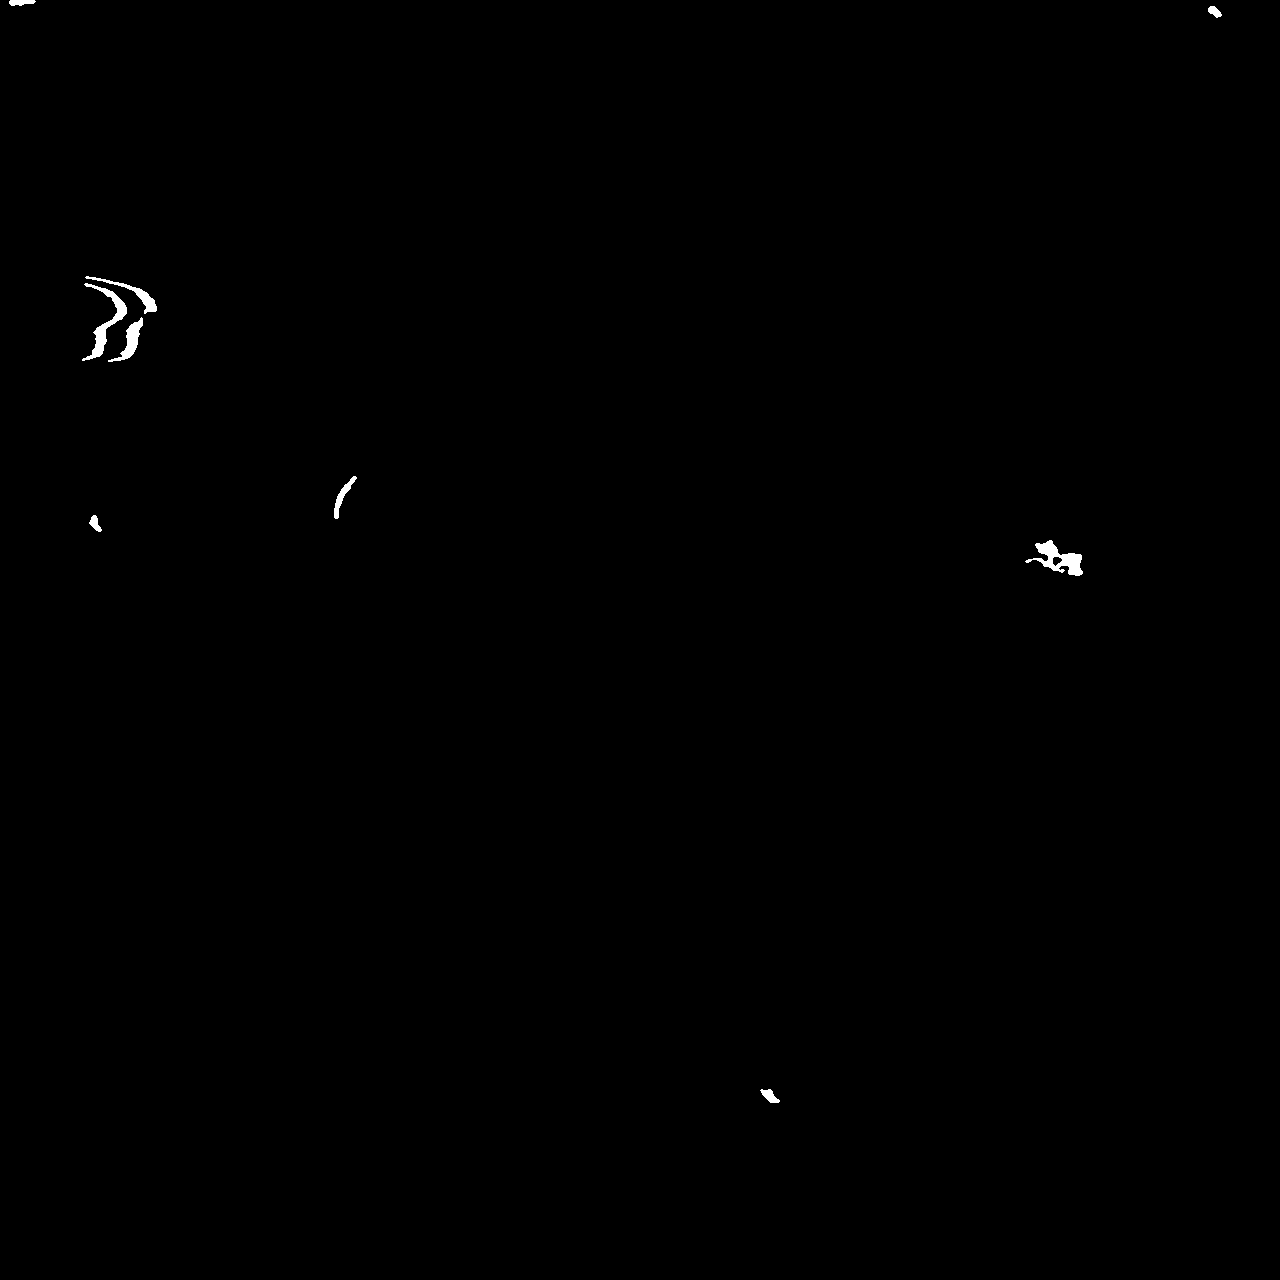
\includegraphics[width=\linewidth]{before.png}
		\caption{Before}
		\label{fig:bwbefore}
	\end{subfigure}%
	\hspace{\fill}
	\begin{subfigure}{0.5\textwidth}
		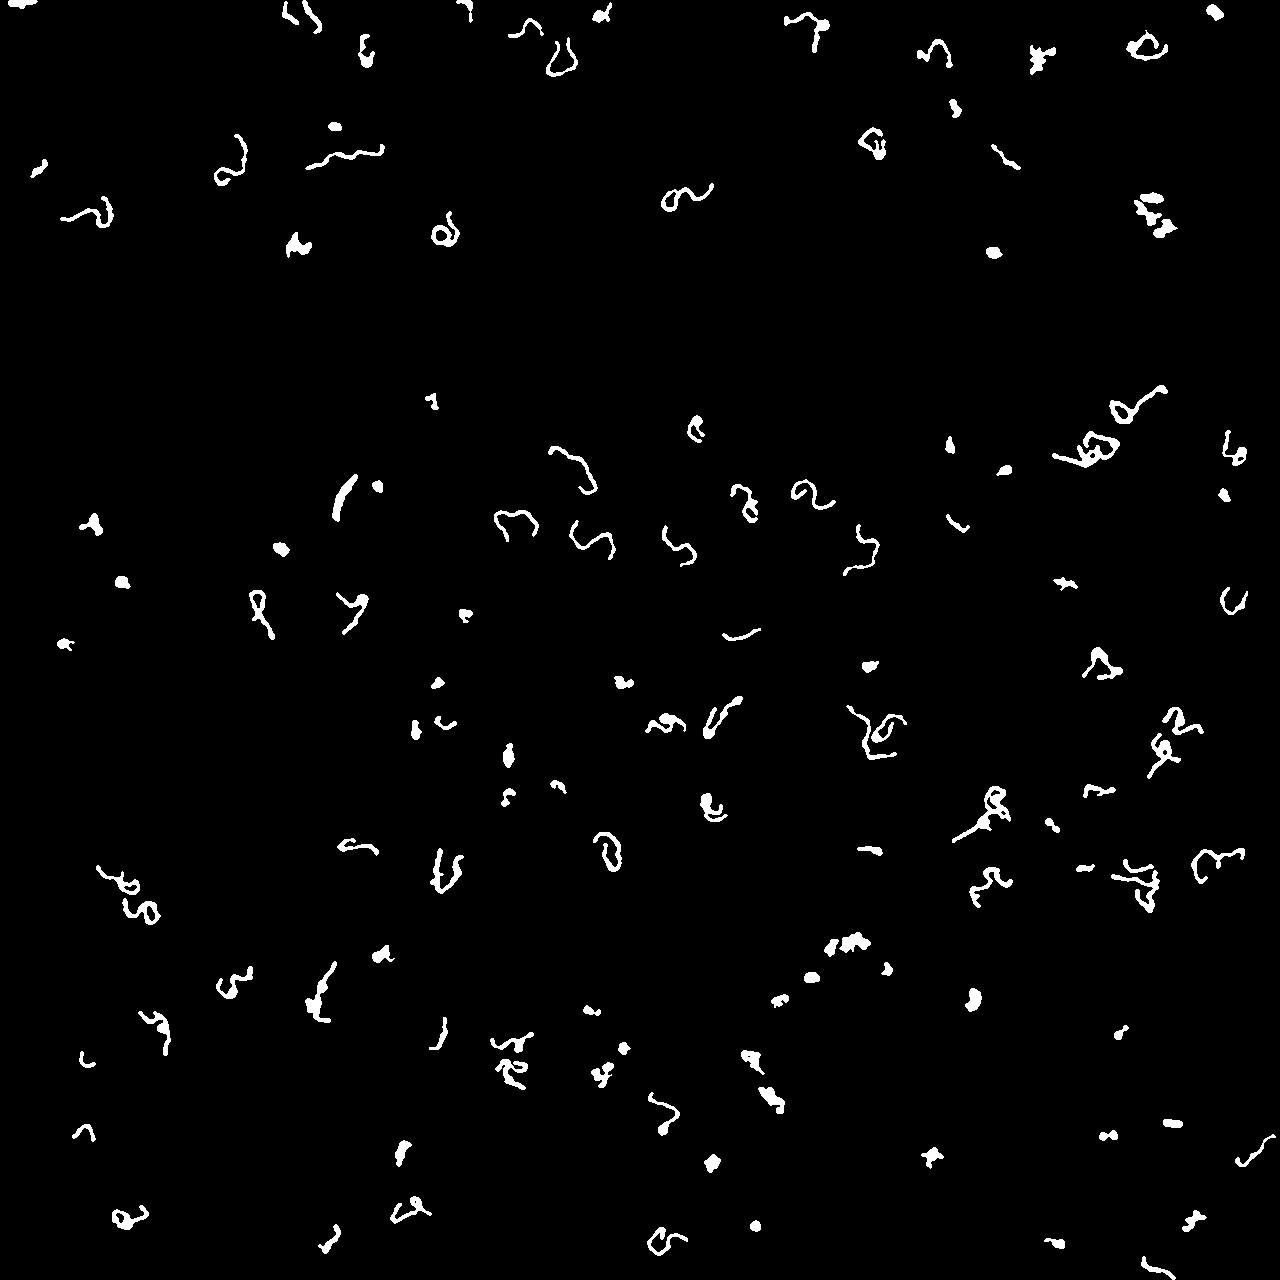
\includegraphics[width=\linewidth]{after.png}
		\caption{After}
		\label{fig:bwafter}
	\end{subfigure}%
	\caption{Comparison with previous method, noise type 1}\label{fig:compareThresh}
\end{figure}

\subsubsection{Limit Threshold}
The first two steps focused on keeping the noise and distribution of the height values in a tolerable range on image to image basis. The third and final step of this method aims at limiting the thresholds over the entire dataset.
For this technique a larger dataset of at least 50 images is required.
The histogram of all 105 test images shown in Figure \ref{fig:HistogramThresholds} shows that step one and two already improve the thresholds to a smaller range.
Also, only thresholds, which were too high, have been limited by these steps since only outliers in the upper value range have been treated, while lower values have been set to a fixed background.
The newly calculated thresholds are in a range between 0.4 and 0.46 which corresponds to pixel values of 102 and 117.
Looking at the images with the highest and lowest thresholds, it turns out that they are still prioritizing lower respectively higher pixel values. This results in too small DNA-strands or false positive detections.
In order to limit the probability of these cases the permissible range for thresholds is reduced even further. This is achieved by only allowing thresholds in the range of 1.5 times the standard deviation around the mean of the distribution.
The range is thereby limited to: 
\[
[\bar X - 1.5 * \sigma, \bar X + 1.5 * \sigma] 
\]
\[
= [0.4345-1.5*0.0129, 0.4345+1.5*0.0129] 
= [0.4152,0.4538]\,  % Formel allgemein hinzufügen
\]
All values outside of this interval are set to the nearest boundary.



\begin{figure}[!htb]
	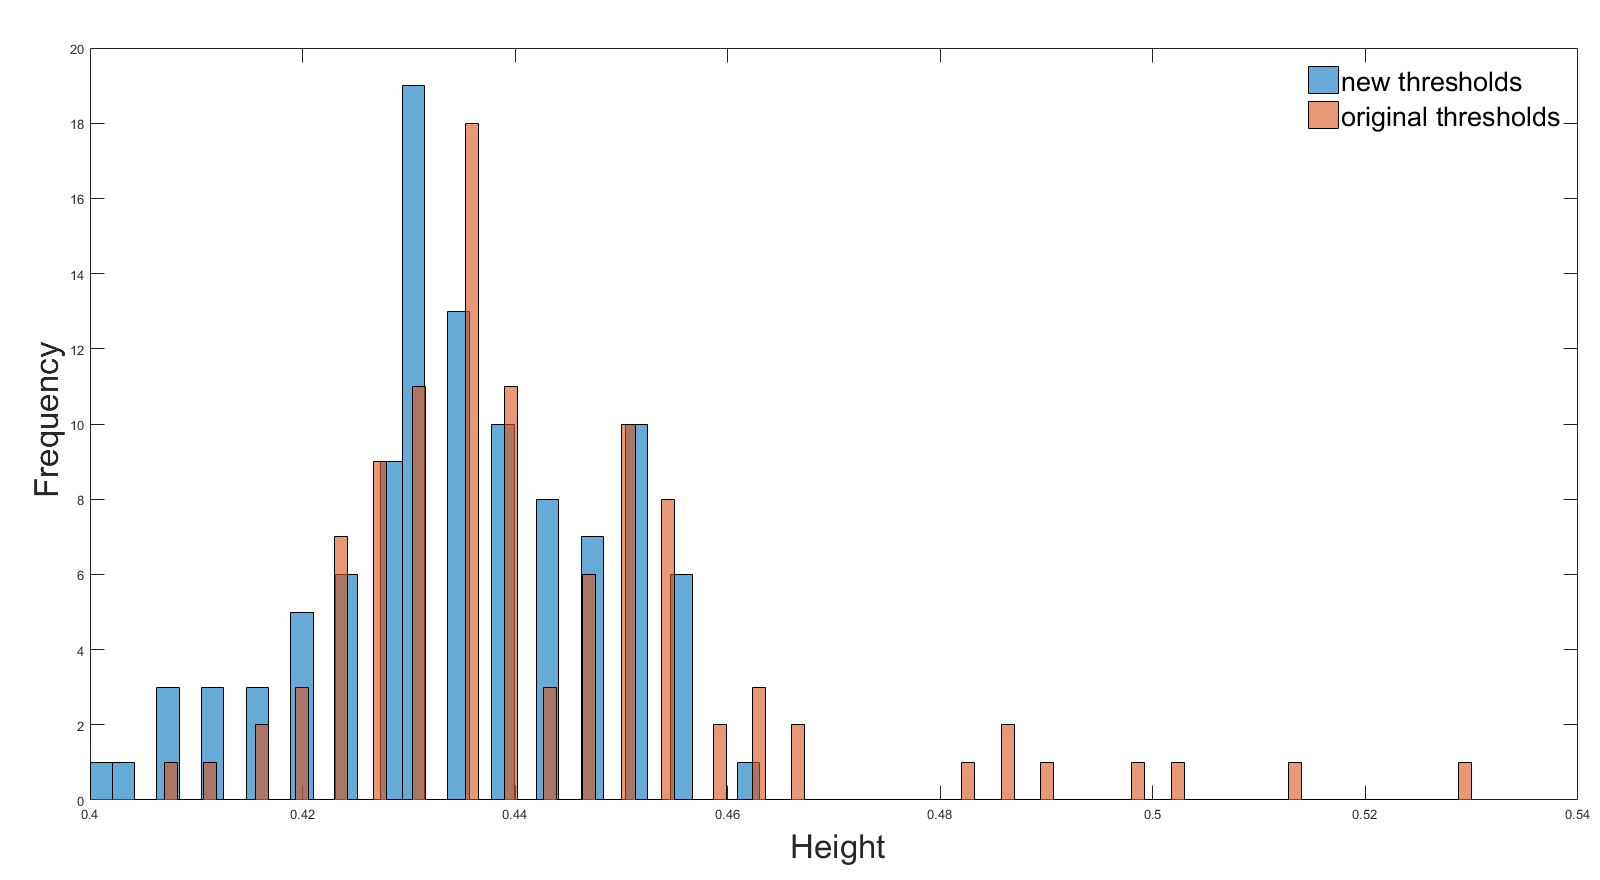
\includegraphics[width=1\linewidth]{thresholds.png}
	\caption{Threshold Distribution over the entire dataset (orange)before and (blue)after step one and two were applied}%formulierung ändern
	\label{fig:HistogramThresholds}
	\end{figure}
	As seen in Figure \ref{fig:compareThresh} this method effectively detects and removes polluted image regions and ensures a high DNA-strand detection on images with noise type one.
Due to the nature and height field of noise of type two this approach can only limit false detections to a certain degree (see Figure \ref{fig:compareThresh1}).
Although it was not expected to work on this kind of imperfections at all. While almost all DNA-strands are detected correctly some false positive still exist.
In conclusion, the proposed approach improves image quality and detection rate on very noisy images greatly while leaving already well processed images the way they are.

\begin{figure}[!htbp]
	\begin{subfigure}{0.5\textwidth}
		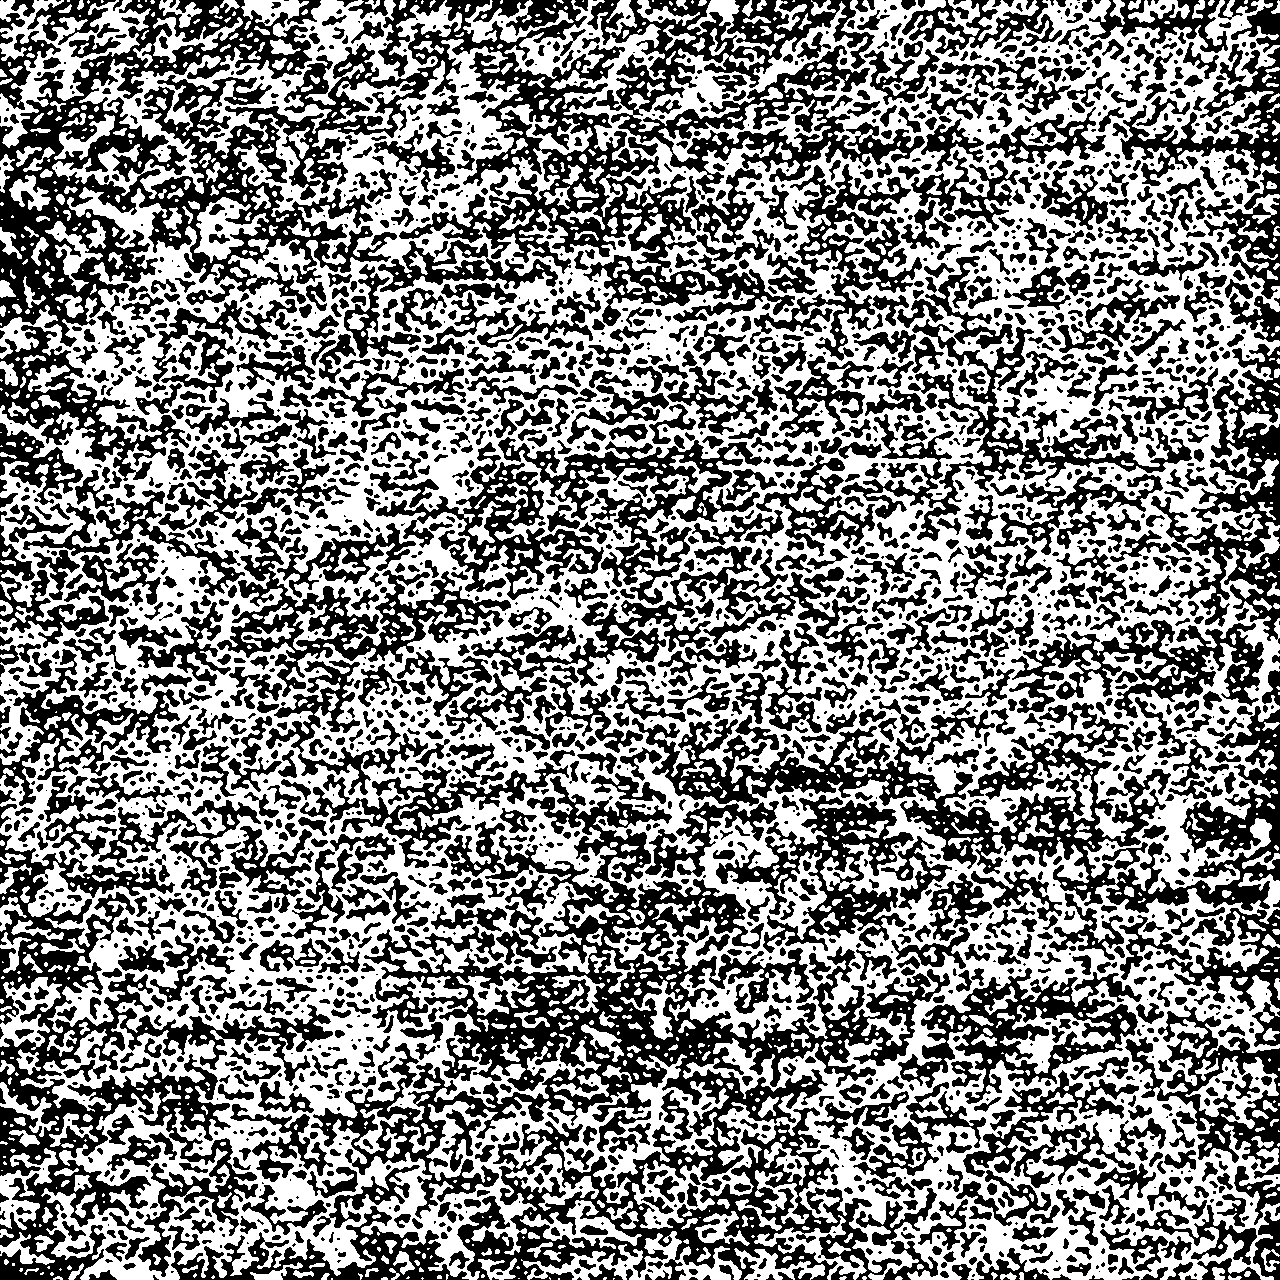
\includegraphics[width=\linewidth]{noise2before.png}
		\caption{Before}
		\label{fig:bwbefore}
	\end{subfigure}%
	\hspace{\fill}
	\begin{subfigure}{0.5\textwidth}
		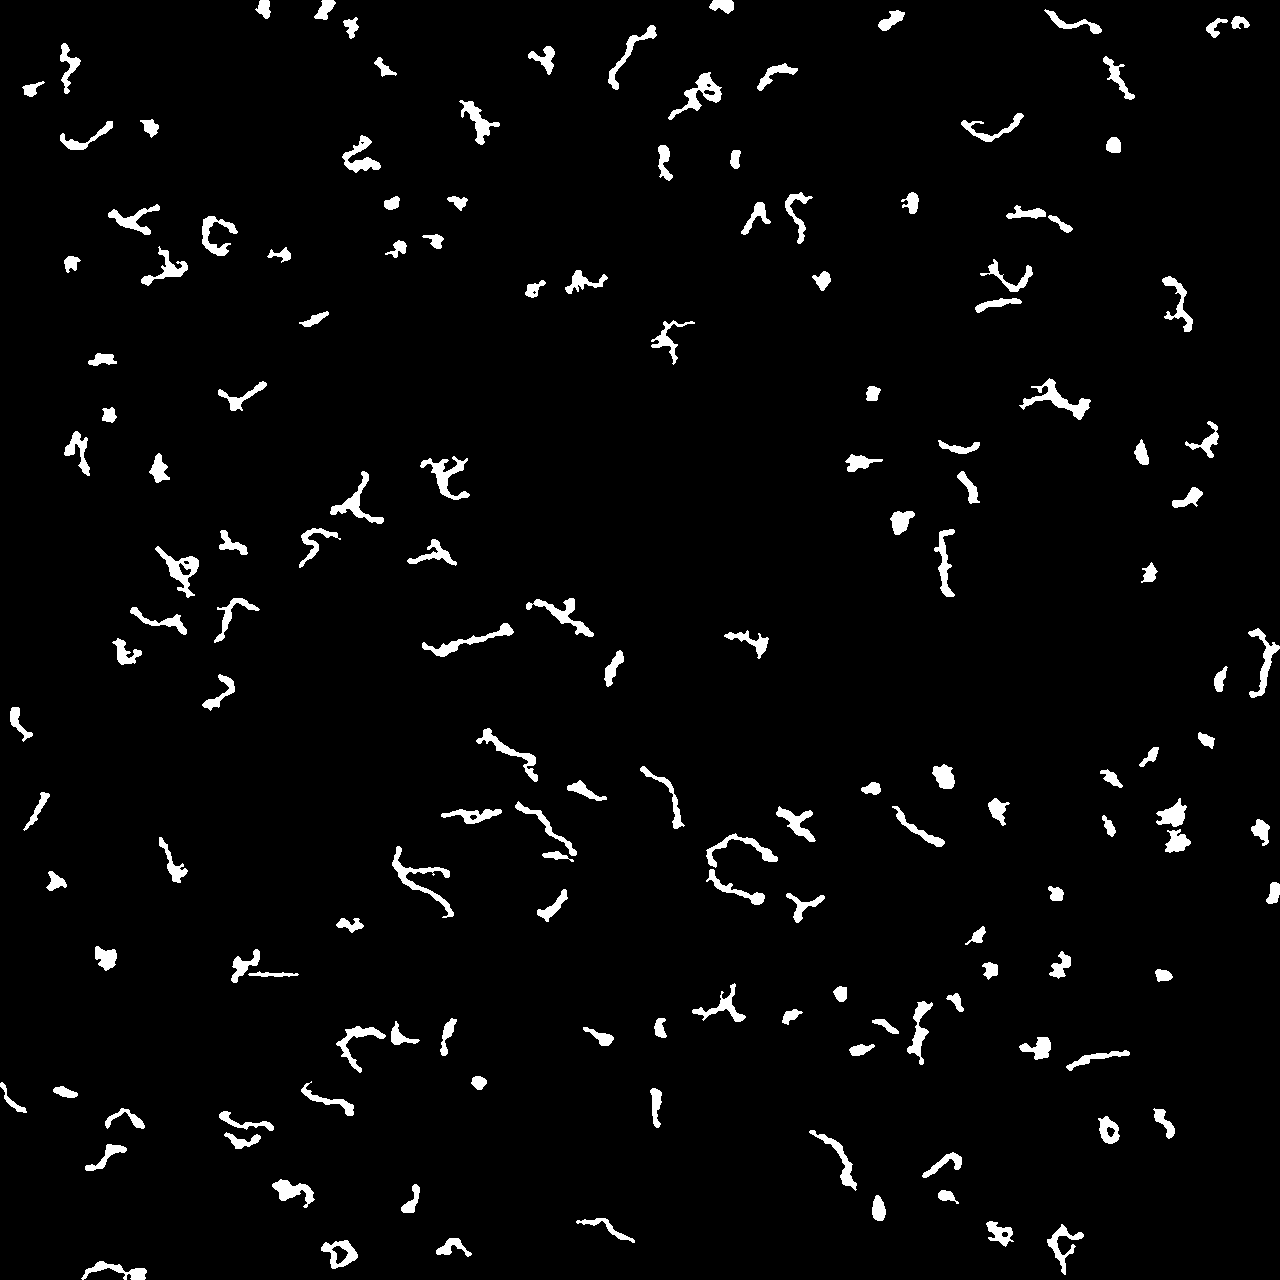
\includegraphics[width=\linewidth]{noise2after.png}
		\caption{After}
		\label{fig:bwafter}
	\end{subfigure}%
	\caption{Comparison with previous method, noise type 2}\label{fig:compareThresh1}
\end{figure}
\newpage

\subsection{Nucleosome Detection}\label{sec:Nucleosome Detection}
To determine whether the DNA contains a nucleosome and to measure the angle of the two branches wrapped around the nucleosome, an algorithm for nucleosome detection has been implemented. Due to the nucleosomes's appearance, an algorithm to detect bright circles with center $(i,j)$ and radius $r$, defined by
\begin{align}\label{eq: circle}
(x -i)^2+(y-j)^2 = r^2 
\end{align}
has been chosen, the MATLAB imfindcircles function. It is based on a Circular Hough Transform which provides robustness in the presence of noise, occlusion and varying illumination. Votes are cast in the Hough space which is made up of a cell for each pixel. Initially each cell is set to 0.

The algorithm considers foreground pixels that have a high image gradient value as candidates for the edges of a circle. For the image data in this project the foreground pixels are bright pixels. As the nucleosomes in the AFM images are blurry and of low contrast in relation to the background, their edges are weak and thus the image gradient threshold value has to be set relatively low. Each edge candidate pixel $p_{edge}=(x,y)$ is then the center point to a voting circle of a radius $r$, meaning that each edge candiate pixel casts votes in the Hough space to the bins $b = (i,j)$ which according to equation \ref{eq: circle} could be the center of the circle and therewith the center of the nucleosome.

The point where locally most voting circles coincide, which equals the bin in Hough space where votes accumulate, is marked as the center point of the actual circle, see Figure \ref{fig: houghTransfom1}. 

\begin{figure}[htb!]
\centering
\def\svgwidth{0.95\textwidth}
\input{houghTransfom1.pdf_tex}
\caption{Left: A voting circle (dashed) has its center point at a pixel of high gradient, e.g. on the actual circle's edge. Right: The actual circle that is to be detected (solid) is centered around the point where most voting circles meet.}\label{fig: houghTransfom1}
\end{figure}

However, the nucleosomes have different radii ranging between 4 and 6 pixels, such that the voting has to be done for several different radii leading to not just intersecting circles, but intersecting cones, see Figure \ref{fig: houghTransfom2}.

\begin{figure}[htb!]
\centering
\def\svgwidth{0.95\textwidth}
\input{houghTransfom2.pdf_tex}
\caption{Left: If the radius is unknown, votes will be cast not just to one circle but to many circles of radii $r$ in a given range.  Right: Voting circles of different radii add up to voting cones in Hough space.}\label{fig: houghTransfom2}
\end{figure}

As the image gradient direction is known, the problem is slimmed down to intersecting lines in the Hough space instead of the intersecting cones, see Figure \ref{fig: houghTransfom3}.
This is possible because the gradient direction tells the exact direction in which the center of the circle has to lie and subsequently one does not have to vote for a whole circle of possible center locations but just a single point or respectively for unknown radii, a line. The radius and circle center location is then given by the bin with the most votes, that is where most of the lines intersect.
%The corresponding radius is then estimated based on computing radial histograms. CHECK EXPLAIN

\begin{figure}[htb!]
\centering
\def\svgwidth{0.95\textwidth}
\input{houghTransfom3.pdf_tex}
\caption{Left: The image gradient gives information as to where the center of the actual circle is placed, hence votes are cast to just a point not to a circle. Right: Voting points for different radii add up to a voting line in Hough space.}\label{fig: houghTransfom3}
\end{figure}

 % [1] T.J Atherton, D.J. Kerbyson. "Size invariant circle detection." Image and Vision Computing. Volume 17, Number 11, 1999, pp. 795-803.
%[2] H.K Yuen, .J. Princen, J. Illingworth, and J. Kittler. "Comparative study of Hough transform methods for circle finding." Image and Vision Computing. Volume 8, Number 1, 1990, pp. 71–77.

%\begin{figure}[htb!]
%\centering
%\def\svgwidth{0.95\textwidth}
%\input{houghTransfom1.pdf_tex}
%\def\svgwidth{0.95\textwidth}
%\input{houghTransfom2.pdf_tex}
%\def\svgwidth{0.95\textwidth}
%\input{houghTransfom3.pdf_tex}
%\caption{\textbf{First row}: A voting circle (dashed) has its center point at a pixel of high gradient, therewith on the actual circle's edge. The actual circle that is to be detected (solid) is centered around the point in which most voting circles meet. \textbf{Second row}: If the radius is unknown, votes will be cast not just to one circle but many circles of radii $r$ in a given range.  Voting circles of different radii add up to voting cones in Hough space.\textbf{ Third row}: The gradient gives information as to where the center of the actual circle is placed, thus it is voted for a point instead of a circle. Right: Voting points for different radii add up to a voting line in Hough space.}\label{fig: houghTransfom}
%\end{figure}

Applying this method, the nucleosomes as well as noise of circular shape was detected. As only nucleosomes that are located on a DNA strand are of interest, the other detected circles can be dropped. This is done checking the pixel intensity value of the center points of all detected circles in the binary images. In those images noise is already deleted, such that the circles that were fitted to noise will have a pixel intensity value of zero at their center point. Thus, only circles with a non-zero pixel intensity value are considered as nucleosomes, see Figure \ref{fig: find nukleii}.

\begin{figure}[h!]
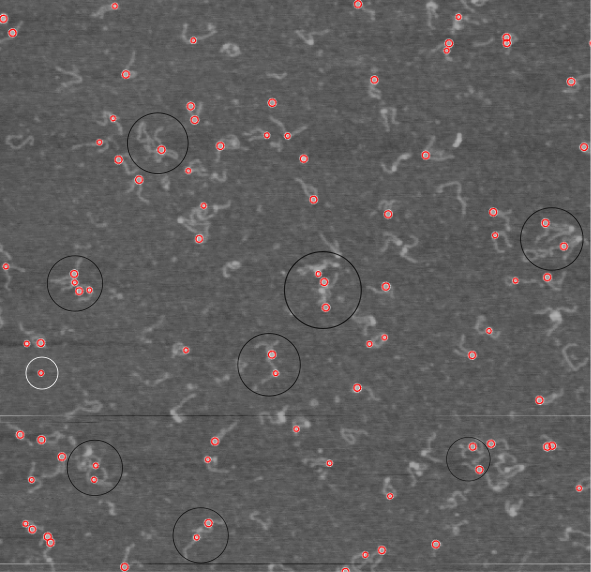
\includegraphics[width =0.5\textwidth]{findNukleii_rawCloseAn}
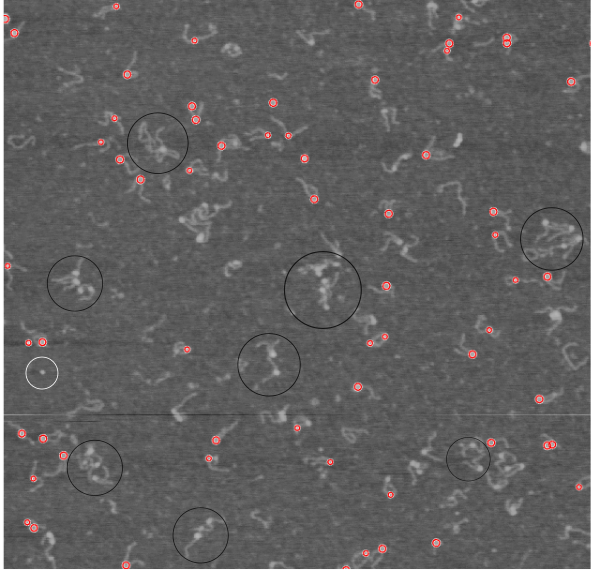
\includegraphics[width =0.5\textwidth]{findNukleii1_rawCloseAn}
\caption{Left: All detected nucleosomes are shown as red circles. Right: The detected nucleosomes after dropping those on overly big DNA strands (marked with black circles) and noise (marked with a white circle).} \label{fig: find nukleii}
\end{figure}
\newpage



\subsection{Thinning}\label{sec:Thinning} % sources: http://cgm.cs.mcgill.ca/~godfried/teaching/projects97/azar/skeleton.html, leelam
To obtain an accurate length measurement, the center line of the DNA is extracted. This is done by thinning the segmented DNA down to a single pixel width line corresponding to the skeleton of the DNA which can then be further processed for length and angle measurement. Two thinning algorithms have been tested in the scope of the project.



\subsubsection{Hilditch's Sequential Thinning}\label{sec:Hilditch's Sequential Thinning}
The first method is based on Hilditch's sequential thinning algorithm   \cite{lam1992thinning} and is implemented via MATLAB's \verb|bwmorph| function. For each DNA pixel $p$ the 8-neighborhood $N(p)$ is considered when deciding whether to disregard the pixel or keep it as part of the resulting skeleton. The neighborhood $N(p)$ includes the points $x_i, i= 1,\dots 8$ starting from the point east of pixel $p$ and counting upwards counterclockwise, compare Figure \ref{tab: neighborhood}. Their values correspond to the pixel intensity, such that
\begin{align*}
x_i = \begin{cases}
1 & \text{if } x_i \text{ is a DNA pixel}\\
0 & \text{if }x_i \text{ is a background pixel}
\end{cases}\, .
\end{align*}

\begin{figure}[htb]
\centering
\renewcommand{\arraystretch}{2}
\begin{tabular}{|c|c|c|}\hline
$x_4$ & $x_3$ & $x_2$ \\\hline
$x_5$ & $p$ & $x_1$ \\\hline
$x_6$ & $x_7$ & $x_8$\\\hline
\end{tabular}
\caption{8-Neighborhood of pixel $p$.}\label{tab: neighborhood}
\end{figure}

The pixels $p$ are scanned from left to right and top to bottom and are considered for deletion if they satisfy the following properties:
\begin{enumerate}
\item $p$ is a white pixel.
\item $p$ is not an isolated or end point
\item $p$ is a contour pixel, i.e., $p$ has at least one black 4-neighbor.
\end{enumerate}
For all those pixels, the algorithm performs two sub-iterations. In the sub-iterations pixel $p$ is deleted if the following conditions hold:
\begin{itemize}
\item \textbf{Condition 1} There is exactly one white connected component including white 4-neighbor pixels in $N(p)$:
\begin{equation*}
X_H(p)=1, 
\end{equation*}
where the crossing number $X_H(p)$ is the number of white connected components in $N(p)$:
\begin{align*}
& X_H(p) = \sum_{i=1}^4 b_i,\\\nonumber
& \text{where }
b_i=\begin{cases}
1 & \text{if } x_{2i-1} \wedge (\overline{x}_{2i} \vee \overline{x}_{2i+1})\\
0 & \text{else}
\end{cases} \\
\end{align*}
and where $x_i$ are the pixels in the neighborhood $N(p)$ as defined above and the pixel values are treated as boolean values such that $\overline{x}_i$ is the negation of $x_i$.
% DNA pixels are white, such that their value $x_i=1$, background pixels black and therewith $x_i = 0$. 

\item \textbf{Condition 2} Pixel $p$ is not an endpoint, branch point or isolated pixel and has to be a boundary pixel:
\begin{equation*}
2\leq \min\{n_1(p), n_2(p)\} \leq 3,
\end{equation*}
where
\begin{align*}
n_1(p) = \sum_{k=1}^4 \overline{x}_{2k-1}\vee \overline{x}_{2k}\\
n_2(p) = \sum_{k=1}^4 \overline{x}_{2k}\vee \overline{x}_{2k+1}
\end{align*}
\item \textbf{Condition 3} One pixel wide vertical and horizontal lines are not eroded by deletion of pixel $p$.
\begin{itemize}
\item First sub-iteration: $(x_2 \wedge x_3 \wedge \overline{x}_8) \vee x_1$
\item Second sub-iteration: $(x_6 \wedge x_7 \wedge \overline{x}_4) \vee x_5$
\end{itemize}
\end{itemize}
The two sub-iterations are repeated until the image stops changing. The result are one-pixel-wide ridges representing the center lines of the DNA strands, see Figure \ref{fig: thinning}. It can be observed that noise as well as the nucleosomes result in little branches on the center line. The branches are not needed for the calculation of the DNA's length such that they have to be removed, see Section \ref{sec:Erosion of Noise Branches}.

\begin{figure}[htb]
\centering
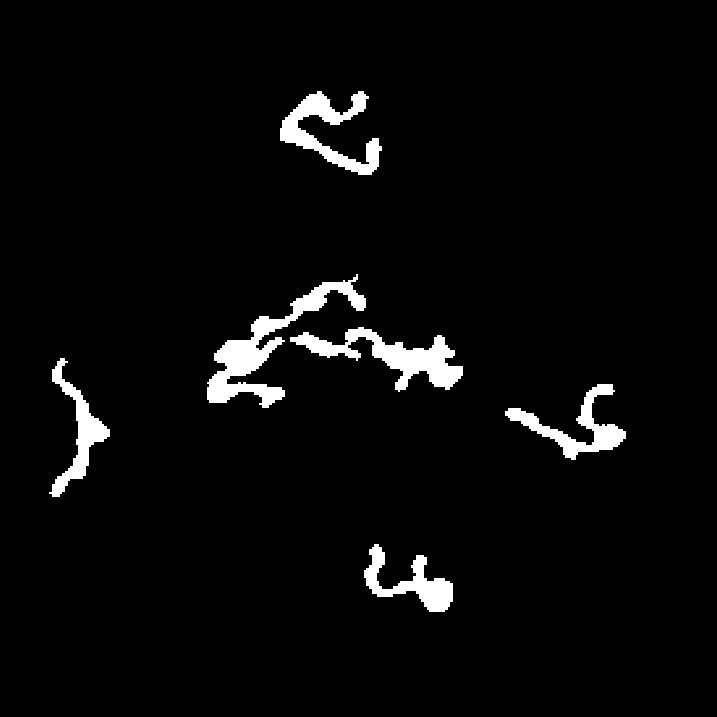
\includegraphics[width = 0.49\textwidth]{bin.png}
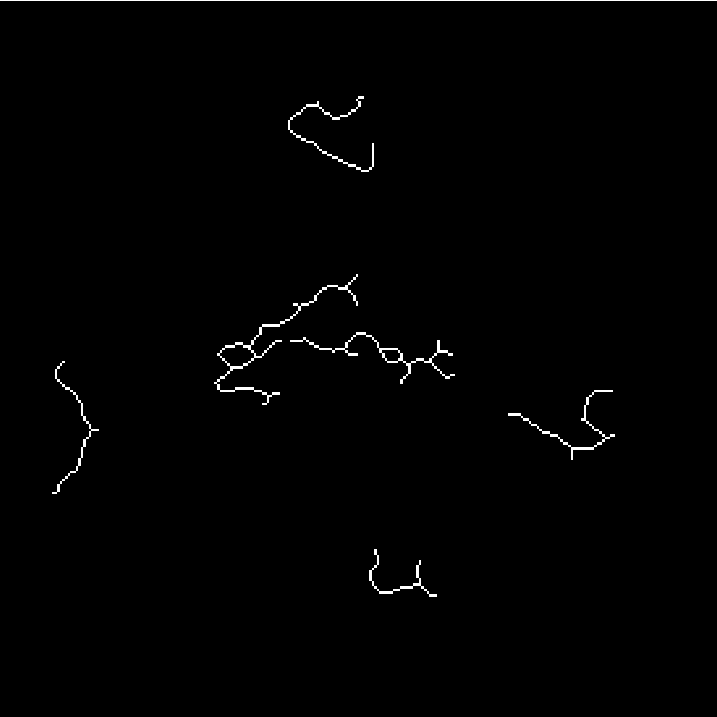
\includegraphics[width = 0.49\textwidth]{thinned.png}
\caption{Section of an AFM image after segmentation and binarization (left) and after thinning (right).}
\label{fig: thinning}
\end{figure}
\subsubsection{Zhang Suen Parallel Thinning}\label{sec:Zhang Suen Parallel Thinning}
The second method is the Zhang Suen thinning algorithm \cite{zhang1984fast} following the implementation given in \cite{linbo2013implementation}. It can be used to attenuate various types of digital patterns   \cite{widiarti2011comparing}.
Since it is a parallel method, the new value for any pixel can be computed using only the 8-neighborhood $N(p)$ values known from the previous iteration.
The contour pixels are deleted in two sub-iterations until no more changes occur in the image and a one-pixel wide 8-connected skeleton is obtained. A DNA pixel is deleted by setting its value to zero, the label of the background pixels.
Pixel $p$ is deleted, if the following conditions hold:
\begin{itemize}
\item \textbf{Condition 1} There is exactly one white connected component in $N(p)$:
\begin{align*}
A(p) = 1\, ,
\end{align*}
where $A(p)$ is the number of white to black crossings in the ordered set $x_1,x_2,\dots, x_8$ of $N(p)$.
\item \textbf{Condition 2} Pixel $p$ is not an endpoint or isolated pixel and has to be a boundary pixel:
\begin{equation*}
2 < n(p) < 6,
\end{equation*}
where $n(p)$ is the number of nonzero neighbors of $p$:
\begin{align*}
n(p) = \sum_{i=1}^8 x_i
\end{align*}
\item \textbf{Condition 3}
\begin{itemize}
\item First sub-iteration: Pixel $p$ is either a south-east boundary point or a north-west corner point. \begin{align*}
\overline{x}_1 \vee \overline{x}_7 \vee (\overline{x}_3  \wedge \overline{x}_5)
\end{align*}
\item Second sub-iteration: Pixel $p$ is either a north-west boundary point or a south-east corner point. \begin{align*}
\overline{x}_3 \vee \overline{x}_5 \vee (\overline{x}_1 \wedge \overline{x}_7)
\end{align*} 
\end{itemize}
\end{itemize}

The result of this algorithm differs from the result of Hilditch's algorithm as can be seen in Figure \ref{fig: thinnedHilditchZhang}. The center lines extracted with Hilditch's algorithm are smoother than the Zhang Suen algorithm. Further differences are discussed in Section \ref{sec: Results}.
\begin{figure}[htb!]
\centering
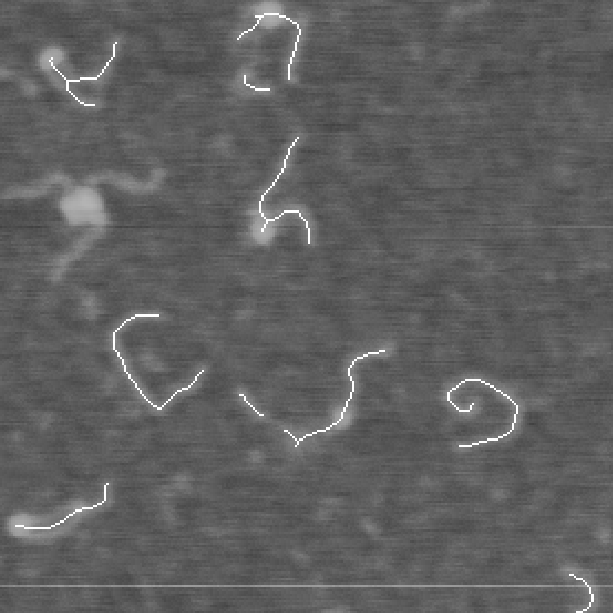
\includegraphics[width = 0.4\textwidth]{thinnedHilditch.png}
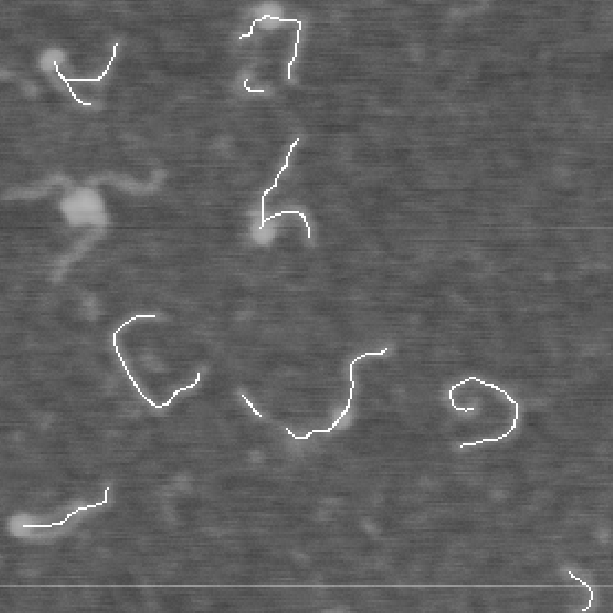
\includegraphics[width = 0.4\textwidth]{thinnedZhangSuen.png}
\caption{An AFM image section overlayed with the thinned DNA strands in white. Result of Hilditch's Sequential Thinning algorithm (left) and result of the Zhang Suen algorithm (right).}
\label{fig: thinnedHilditchZhang}
\end{figure}
\newpage
% second approach: Zhang-Suen https://github.com/linbojin/Skeletonization-by-Zhang-Suen-Thinning-Algorithm/blob/master/thinning.m
\subsection{Erosion of Noise Branches}\label{sec:Erosion of Noise Branches}
\subsection{Lenght Estimation}
\subsection{Angle Measurement}\label{sec:Angle Measurement}
For the DNA strands with a nucleosome, the angle between the two DNA branches is measured. DNA strands with more than one nucleosome will not be assigned an angle measurement neither will DNA strands without nucleosome. Furthermore, if the nucleosome is positioned at the end of the DNA strand as depicted in Figure \ref{fig: angle not}, the angle cannot be measured either. 
\begin{figure}[htb]
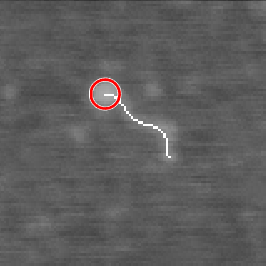
\includegraphics[width = 0.49\textwidth]{angle_endstrand.png}
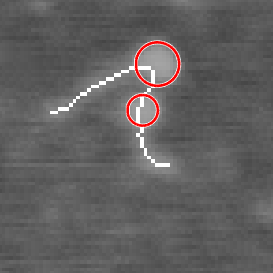
\includegraphics[width = 0.49\textwidth]{angle_two.png}
\caption{DNA strand with the nucleosome on the strand end (left) and more than one detected nucleosome (right). These cases are not considered for angle measurement.}\label{fig: angle not}
\end{figure}

To discard those cases a mask is set up which is zero at all pixels belonging to the nucleosome and one elsewhere. Multiplication of the mask with the image of the DNA's center line, that is the thinned DNA after erosion of all branches, leads to an image of the DNA branches. After applying a connected component analysis each branch is represented by one connected component. All samples with a number of connected components unequal to two will be dropped and only the remaining samples with two connected components, respectively branches, are considered for the angle measurement.
Two ways to measure the angle between the two branches of the DNA have been implemented in the scope of this project.

\subsubsection{Measurement over Nucleosome Center}\label{sec:Measurement over Nucleosome Center}
The first method for the angle measurement is to determine the intersection of the DNA branches and the circle fitted to the nucleosome, draw one line from each intersecting point to the nucleosome center and then calculate the angle between those two lines. This approach has been described in \cite{bussiek2005dna}.
To determine the intersection of the DNA branches with the circle fitted to the nucleosome, for both branches the Euclidean distance of each of its pixels to the DNA's nucleosome center $c$ is measured. The pixel with the smallest distance $d$ equals the intersecting pixel points $p$ of this branch.
The angle $\theta$ between the two lines connecting the intersecting points $p_1$ and $p_2$ with the nucleosome center $c$ is calculated by
\begin{align}
\theta &= \arccos{\frac{a\cdot b}{||a||||b||}}\, ,\label{eq: angle}\\
\text{where } a &= c-p_1 \text{ and } b = c-p_2 \, .\nonumber
\end{align}

However, it turned out that the resulting angles are in many cases not representative for the actual branch angles, see Figure \ref{fig: angle1}. 
\begin{figure}[htb!]
\centering
\def\svgwidth{0.5\textwidth}
\input{angle_1.pdf_tex}
\caption{The angle $\theta=\theta_1 = 108^{\circ}$ between the two DNA branches measured with method 1.}\label{fig: angle1}
\end{figure}
\subsubsection{Measurement over Fitted Lines}\label{sec:Measurement over Fitted Lines}
The second method for the angle measurement follows \cite{kepert2003conformation} fitting a line to the first part of a few micrometers of each branch and calculates the angle between those two fitted lines.
The first step is to select the pixels belonging to the first part of the two branches. 

Let \begin{align*}
r_{max} = r+s\, ,
\end{align*}
where $r$ is the nucleosome radius, estimated in Section \ref{sec:Nucleosome Detection} and $s$ is the value determining the size of the first part. A mask which is zero outside of a circle of radius $r_{max}$ around the nucleosome center is applied to the image of the DNA branches leading to the pruned DNA branch stumps.

  Again a connected component analysis is performed on the pixel set, returning two pixel sets, each representing one of the two branch stumps.
The next step is to fit one line to each branch. This is done by computing a least squares polynomial of order one for the given branch points, returning a slope $m$ and an offset $t$ for each branch line.
Subsequently the angle between the two lines is calculated according to Equation (\ref{eq: angle}), which requires the intersecting point $c = [c_x\, c_y]^{\top}$ of the two fitted lines given by:
\begin{align*}
c_x &= -\frac{t_1-t_2}{m_1-m_2}\\
c_y &= m_1 c_x + t_1 = m_2 c_x + t_2\, .
\end{align*}

\begin{figure}[htb!]
\centering
\def\svgwidth{0.5\textwidth}
\input{angle_2.pdf_tex}
\caption{The angle $\theta=\theta_2 = 170^{\circ}$ between the two DNA branches measured with method 2.}\label{fig: angle2}
\end{figure}
%a least squares polynomial 


\subsection{Optimization}\label{sec:Optimization}
\section{Results}\label{sec: Results}
\subsection{Validation}\label{sec:Validation}
\subsection{Biological Significance}\label{sec: Biological Significance}
\section{Discussion}\label{sec: Discussion}
\section{Conclusion and Outlook}\label{sec: Conclusion and Outlook}

\newpage
\bibliography{sources}
\bibliographystyle{unsrt}

\end{document}
